\documentclass[a4paper,12pt]{scrreprt}

%UTF8 rules
\usepackage[utf8]{inputenc}
%ordentlicher Schriftsatz
\usepackage[T1]{fontenc}
%Tabellen- und Bildunterschriften ordentlich formatiert
\usepackage[labelfont=bf, font=small]{caption}
%deutsche Spracheigenheiten wie Umlaute, Abkürzungen und Anführungszeichen
\usepackage[ngerman]{babel}
\usepackage[ngerman]{translator}
\usepackage[babel,strict]{csquotes}

\usepackage{tabularx}
\usepackage{multirow}
\usepackage{booktabs}

\usepackage{amsmath}
\usepackage{siunitx}
%\usepackage{minted}
\usepackage{listings}

\usepackage[gen]{eurosym}

%Bilder
\usepackage{graphicx}
\usepackage{subfig}

\usepackage{listings}

\lstdefinelanguage{JavaScript}{
  keywords={typeof, new, true, false, catch, function, return, null, catch, switch, var, if, in, while, do, else, case, break},
  keywordstyle=\color{blue}\bfseries,
  ndkeywords={class, export, boolean, throw, implements, import, this},
  ndkeywordstyle=\color{darkgray}\bfseries,
  identifierstyle=\color{black},
  sensitive=false,
  comment=[l]{//},
  morecomment=[s]{/*}{*/},
  commentstyle=\color{purple}\ttfamily,
  stringstyle=\color{red}\ttfamily,
  morestring=[b]',
  morestring=[b]"
}
\lstset{
   language=JavaScript,
   backgroundcolor=\color{white},
   extendedchars=true,
   basicstyle=\footnotesize\ttfamily,
   showstringspaces=false,
   showspaces=false,
   tabsize=2,
   breaklines=true,
   showtabs=false,
   captionpos=b
}
%\usepackage{indentfirst}

\usepackage{pgfplots}
\pgfplotsset{compat=1.13}
\usepackage{pgfplotstable}

\usepackage{amssymb}
\usepackage{listings}
\usepackage{xcolor}
%Links etc.
\usepackage{hyperref}
\usepackage{bookmark}
\usepackage{rotating}
\usepackage[style=chicago-authordate,
backend=biber,
bibencoding=utf8]{biblatex}
\addbibresource{Package/literatur.bib}

\usepackage{kmath,kerkis}
\usepackage{tocbasic}
\usepackage[headsepline]{scrlayer-scrpage}
\pagestyle{scrheadings}
\clearpairofpagestyles    
\lohead{\chaptername :\ \leftmark}      
\automark[section]{chapter}                                         
\ofoot[\pagemark]{\pagemark}

\newcommand*{\quelle}{
  \footnotesize Quelle:
}

\newcommand{\ebtteamO}{Sinan Ayhan, Nick Dirlein, Holger Herbersagen}
\newcommand{\ebtteamT}{Marcel Hizli, René Schießwohl}
\newcommand{\ebtstudentid}{188341}
\urldef{\ebtstudentmail}\url{sayhan@stud.hs-heilbronn.de}

\titlehead{
    \begin{flushright}
    
\includegraphics[height=2cm,keepaspectratio]{Bilder/HHN_ab_40_mm_4c_neg.png}
    \end{flushright}
}

\subject{SS2018 Embedded Systems}
\title{LoRa-Messnetzwerk\vfill}
\author{\ebtteamO\\\ebtteamT}

\begin{document}
\pagenumbering{roman}
\maketitle
\newpage

\pagenumbering{arabic}

\pagenumbering{gobble}

\thispagestyle{plain}
\section*{Einleitung}
LoRa ist eine neue innovative Technologie, die sehr energiesparend ist, sodass es perfekt für unsere kommerzielle Idee geeignet ist. 
Die Arbeit zeigt unser Vorgehen und den Verlauf des Projekts innerhalb des Semesters. Hierbei gehen wir sowohl auf die Konzeptionierung, Umsetzung und auf den Ausblick ein. Zudem weiten wir dies aus, indem wir erste Gedanken zur Kommerzialisierung beschreiben. 
In dem folgenden Bild erkennt man unseren ersten fertigen Prototypen und die einzelnen Bauteile, die verwendet wurden. Hierbei handelt es sich um die gelötete Platine, die Wägezelle, das LoRa-Modul mit der Antenne und ein LCD-Display. Detaillierte Informationen zu den einzelnen Bauteilen folgen in den nächsten Kapiteln.
\begin{figure}[H]
    \center
    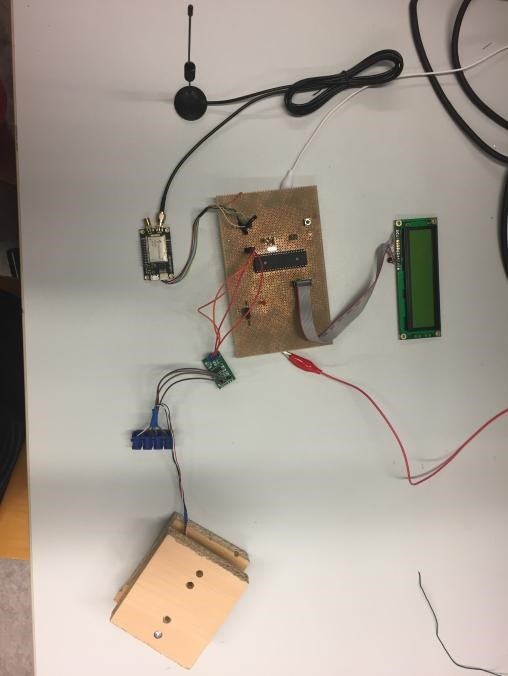
\includegraphics[width=9cm]{Bilder/einleitung.jpg}\\
    \caption{Überblick über die Einzelteile des Prototyps}
    \label{fig:Einleitung}
\end{figure}
\noindent 
Das Ziel dieser Dokumentation ist, dass klar und verständlich erklärt wird, wie der erste Prototyp funktioniert, welche Stärken dieser besitzt und wie man diesen verbessern könnte. 
\newpage

\pagenumbering{roman}
\tableofcontents

\listoffigures

\listoftables
\newpage
\pagenumbering{arabic}

\chapter{Projektvorstellung}
Wir haben uns in der Veranstaltung Embedded Systems des Studiengangs Software-Engineering bei Prof. Dr. Jürgen Doneit und Herr Ulrich Straus im Sommersemester 2018 für das Projekt LoRa-Messnetzwerk entschieden. Die Aufgabe bestand darin, ein Messnetzwerk aufzubauen, welches Sensordaten entgegennimmt und diese über ein Long Range Wide Area Network, kurz LoRaWAN, verschickt.\\
\\
Der daraus resultierende Use-Case:
\begin{figure}[H]
    \center
    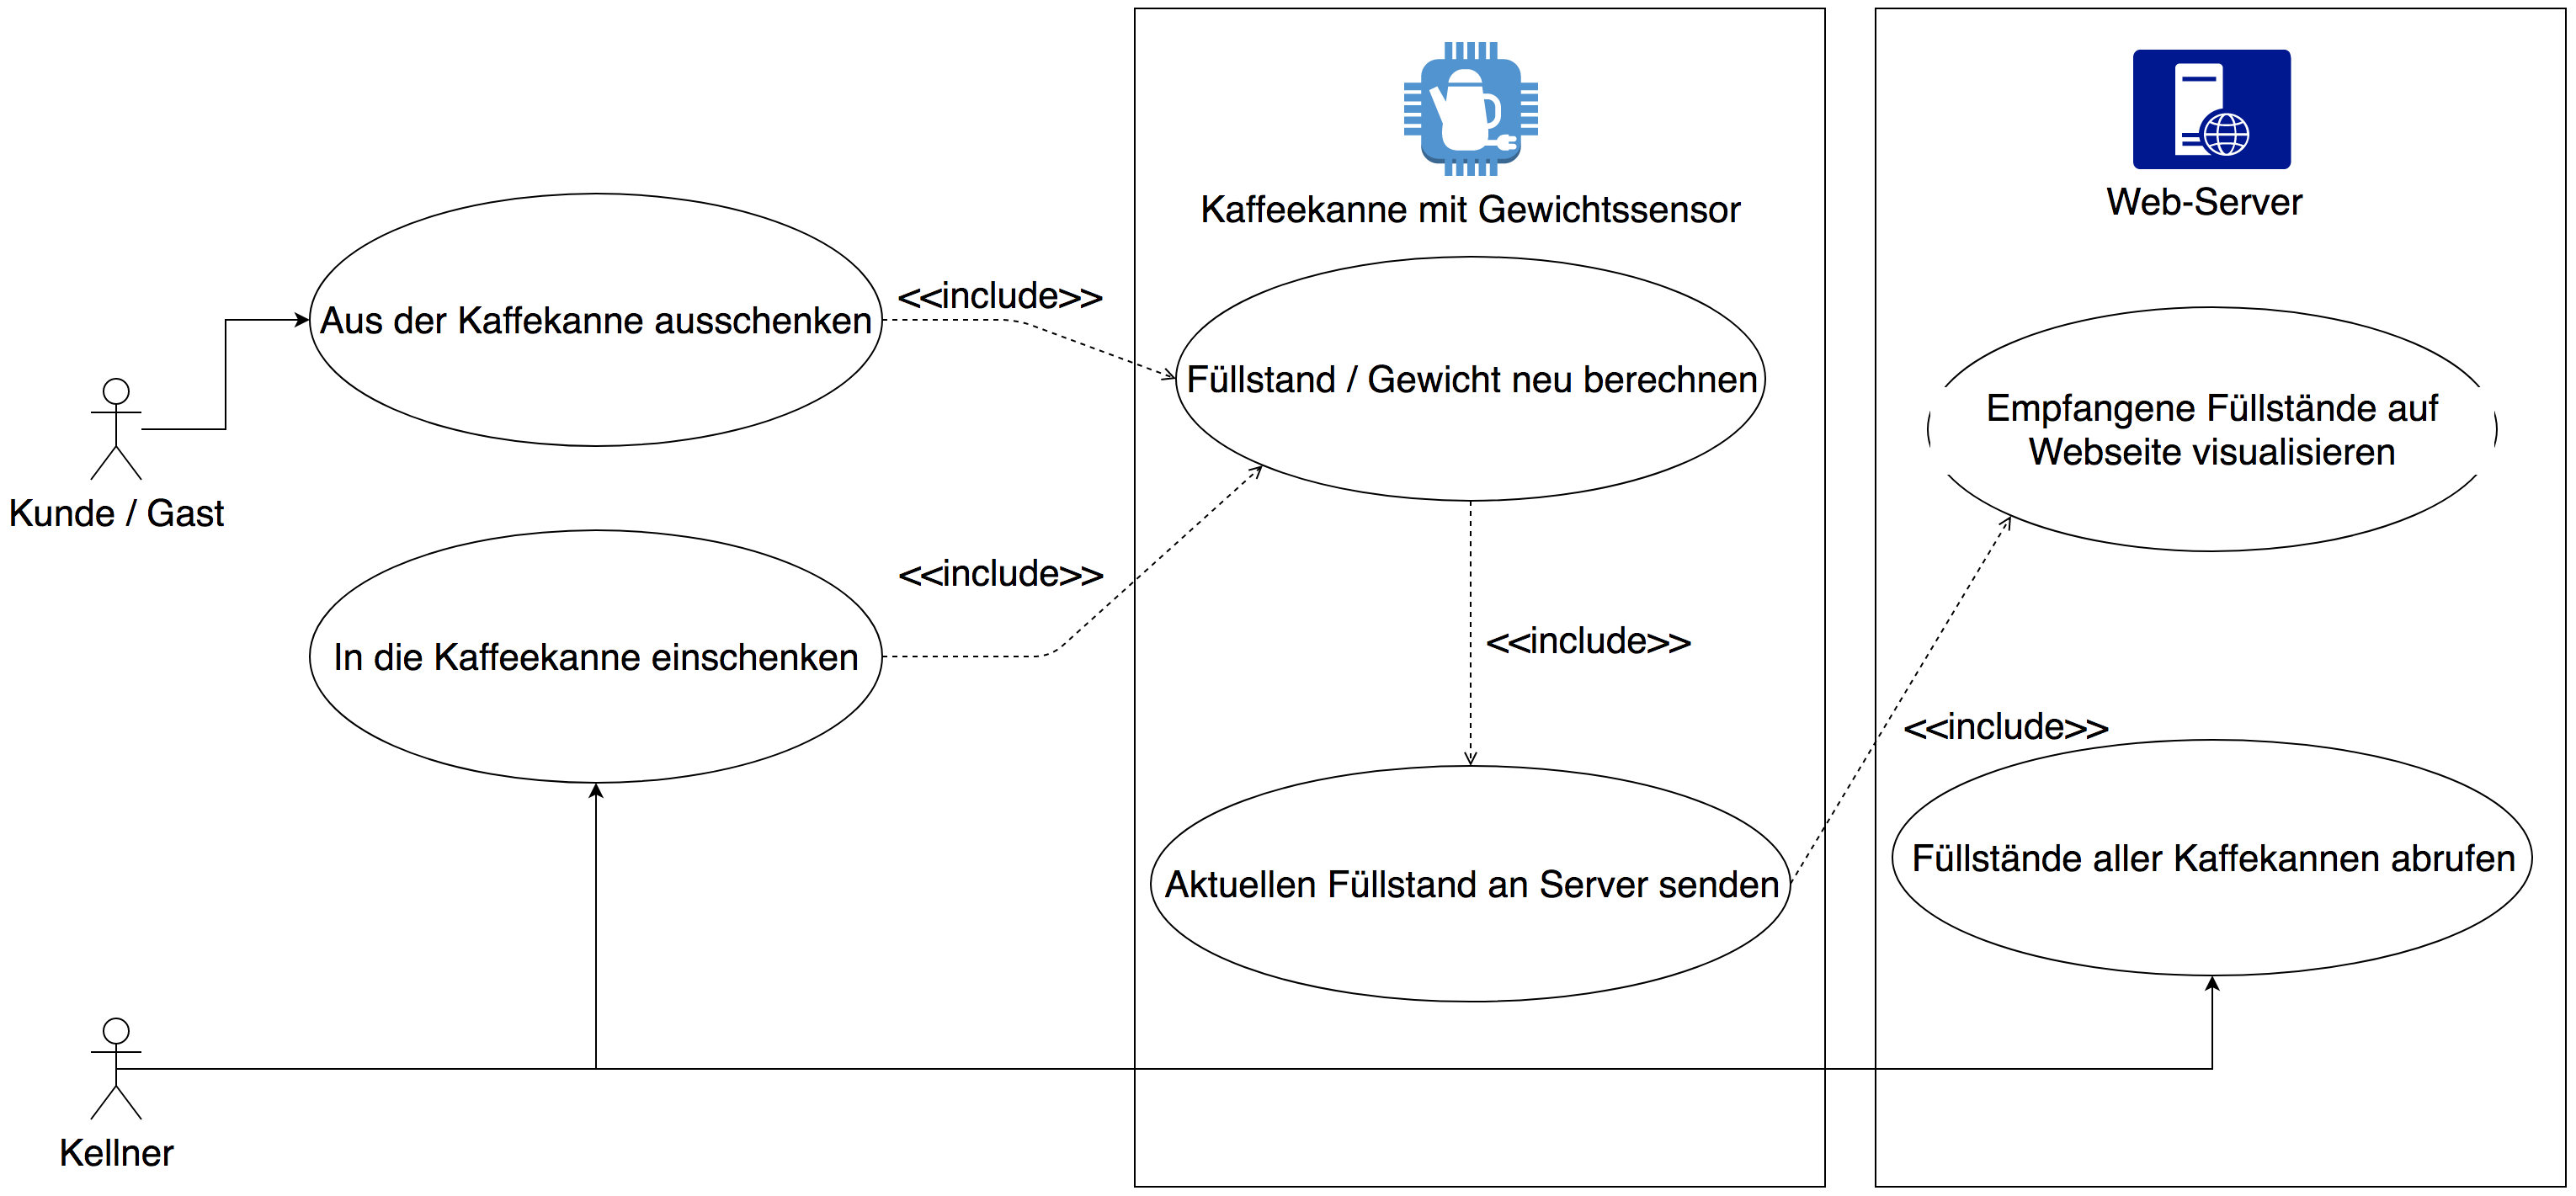
\includegraphics[width=15cm]{Bilder/usecase-1.png}\\
    \caption{Use-Case mit den Akteuren Kunde und Gastronomie-Personal und den Komponenten Kaffeekanne und Web-Server}
    \label{fig:Use-Case}
\end{figure}
\noindent
In einem Restaurant wird der Inhalt einer Kaffeekanne durch das Gewicht bestimmt. Um die Gewichtsmessung für alle Kannen durchzuführen, werden sie auf einer Plattform abgestellt, in der ein Wäge-Sensor-System integriert ist. Das Sensor-System, welches über einen Akku betrieben wird, besteht aus einem Wäge-Sensor, einem Mikrocontroller und einem Transmitter (dem LoRa-Node). Die Messdaten werden jeweils ausgelesen und an den angeschlossenen LoRa-Node übertragen. Die Gesamtheit aller LoRa-Nodes kommunizieren mit einem Empfänger, dem LoRa-Gateway. Das LoRa-Gateway, angeschlossen ans Internet, empfängt die Sensorgewichtsdaten und leitet diese auf einen Web-Server weiter. Das Server-System verarbeitet die Daten, um die Füllstände der Kaffeekannen schlussendlich auf einer Webseite zu visualisieren. Der plattformübergreifende Zugriff über diverse Endgeräte ist somit möglich.

\chapter{Ausgangssituation / Beweggründe für die Umsetzung}
In der Gastronomie üblich, prüft das Personal von Zeit zu Zeit ob in den Behältnissen der Gäste auf den Tischen oder am Buffet noch genügend Inhalt vorhanden ist. Das reicht von der Kaffeekanne auf dem Frühstückstisch, über das Butterbehältnis auf dem Buffett, bis hin zur Weinflasche am Abend im Restaurant. Natürlich gehört dies zum Service eines guten Gastrounternehmens. Auf der anderen Seite kostet es viel Servicekraft die Füllstände zur vollen Zufriedenheit des Kunden und jederzeit im Auge zu behalten.
\\
Unser Ziel ist es bei diesem Prozess eine höhere Effizienz zu erzielen. Es soll zu jeder Zeit und von überall, ohne Sichtprüfung eine klare Aussage über einen nötigen Nachfüllprozess getroffen werden können. Durch das Wegfallen der ständigen Sichtprüfung vor Ort, hat der Kunde eine ruhigere, entspanntere und damit angenehmere Atmosphäre. Er wird nur dann auf den Wunsch des Nachfüllens angesprochen, wenn das Gefäß tatsächlich leer ist. Damit werden deutlich optimalere Geschäftsabläufe gewährleistet: 
\begin{itemize}
    \item Produkte können bedarfsgerechter angerichtet, zubereitet oder hergestellt werden
    \item Wartezeiten gegenüber dem Kunden lassen sich wahrnehmbar verkürzen, die Zufriedenheit steigt
    \item und das Personal kann sich auf andere/wichtigere Themen bezüglich des Kunden konzentrieren
\end{itemize}
Um die Kernfunktionalität im Einsatz zu testen und die Idee zu validieren, beschränken wir uns bei der Entwicklung unseres Prototyps auf die Messung der Füllstände von Kaffeekannen.
\\ 
 Damit das System funktioniert, werden die Kaffeekannen auf einer Plattform abgestellt und durch Wäge-Sensoren gewogen. Die gemessenen Werte und die daraus entstandenen Informationen werden visualisiert und dem Personal über eine Webseite angezeigt. Bei niedrigem Füllstand (oder zu niedriger Temperatur, weil schon zu lange in der Kanne) können sie damit schnell reagieren. Die komplette drahtlose Kommunikation basiert dabei auf LoRa-Nodes, die sehr energiesparend sind. Bei konstanter täglicher Nutzung des Systems ist bei entsprechender Akkugröße eine Laufzeit von einem Jahr möglich. Trotzdem ist zusätzliches Optimierungspotential vorhanden. Denn werden die LoRa-Nodes nach dem Senden der Zeit- und Gewichtsinformationen in einen Sleep-Mode versetzt, zusätzlich der Sende-Zyklus verlängert und serverseitig ein besserer Abstraktionsalgorithmus implementiert, sind bei gleichem Akku Laufzeiten bis zu drei Jahren denkbar.
\\
Am Anfang des Projektes erstellten wir Bauteildiagramme und diskutierten über Kommunikationswege zwischen den Bauteilen. Danach teilten wir Schwerpunkte beziehungsweise Bauteile auf unsere Teammitglieder auf, welche dann nochmal tiefer vom zugewiesenen Teammitglied recherchiert wurden. Die Zusammensetzung der Bauteile erfolgte zunächst um schnelle Validierungstests und Hardwareänderungen durchführen zu können. Nach erfolgreichen Tests auf unserer zuvor zusammengesetzten Entwicklungsplattform wechselten wir die Hardware auf eine selbst konzeptionierte Platine. Mit dem letzten validen Test und nach der offiziellen Präsentation dokumentierten wir unsere Ergebnisse.

\begin{figure}[H]
    \center
    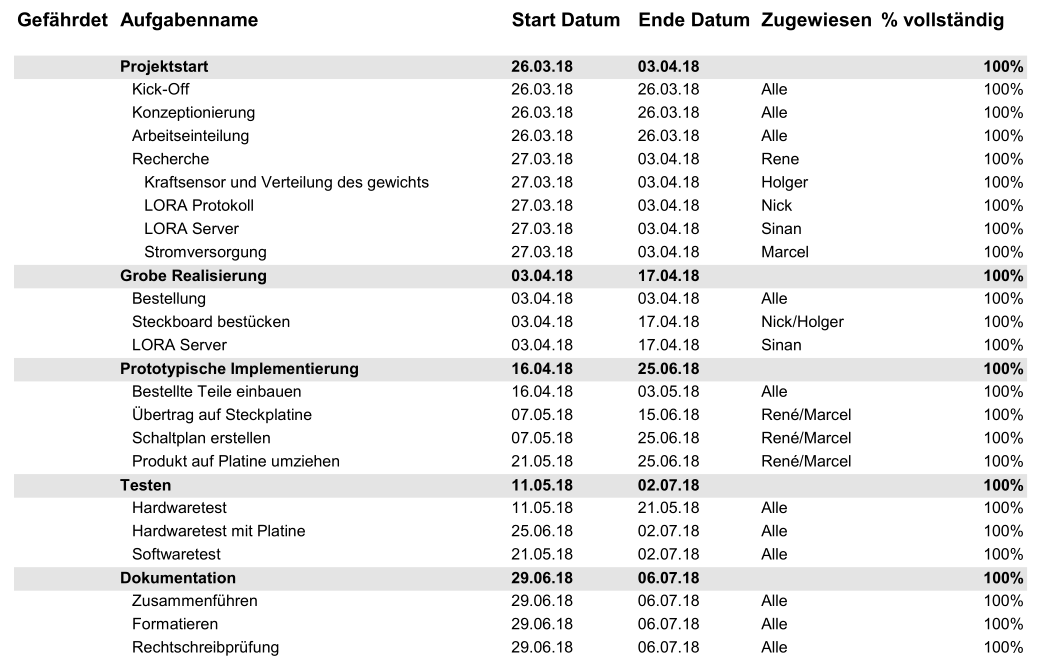
\includegraphics[width=15cm]{Bilder/projektplan.png}\\
    \caption{Projektplan}
    \label{fig:Projektplan}
\end{figure}
\chapter{Einkaufsliste}

\begin{table}[h]
    \caption{Einkaufsliste}
    \centering

    \begin{tabular}{ | l |  l | }
    \hline
    Komponente & Preis \\ \hline
    Web-Server für Node.js  & \\
    VPS oder Cloud Server mieten & ab 5.00 \euro / Monat \\
    oder & \\
    einen vorhandenen, netzwerkfähigen Computer benutzen & - \\ \hline
    LoRa-Gateway iC880A-SPI + Antenne + Pigtail cable + Raspberry Pi 2 B & 167.90 \euro \\ \hline
    LoRa-Node Data Link LoRa RN2483 + Antenne & Ca. 70 \euro \\ \hline
    Wägezelle + HX711 & 10.71 \euro \\ \hline
    Mikrocontroller ATmega644PA & 4.24 \euro \\ \hline
    \end{tabular}
\end{table}
\noindent
Für unseren ersten Prototyp benötigten wir das LoRa-Node Modul mit Antenne, um Daten an das Gateway (Server) verschicken zu können. Außerdem haben wir eine Wägezelle mit einem AD-Wandler (HX711) an einen Mikrocontroller (ATmega644PA) angeschlossen, um damit das Gewicht von der Wägezelle messen und übertragen zu können.\\
Als Vorgriff vor dem Resultat, sei hier an dieser Stelle zu erwähnen, dass während der Validierungstests der Mikrocontroller oder das Steuergerät für die Wägezelle (HX711) als verzichtbar erkannt wurde. Das würde den Preis etwas verringern. Der Grund ist, dass mögliche Sensor-Informationen sich direkt über die Ein- und Ausgangskanäle des LoRa-Moduls (RN2483) ohne Zwischenschritt auf dem Mikrocontroller übertragen lassen. Im weiteren Dokumentationsverlauf wird der Mikrocontroller in Kombination mit dem Steuergerät (HX711) jedoch weiterhin eingesetzt. \\

\chapter{Komponentenmodell des Wägesystems für Kaffeekannen}
Auf dem nachfolgenden Komponentenmodell sind die angedachten Kommunikationswege der einzelnen Module aufgebaut. 
\begin{figure}[H]
    \center
    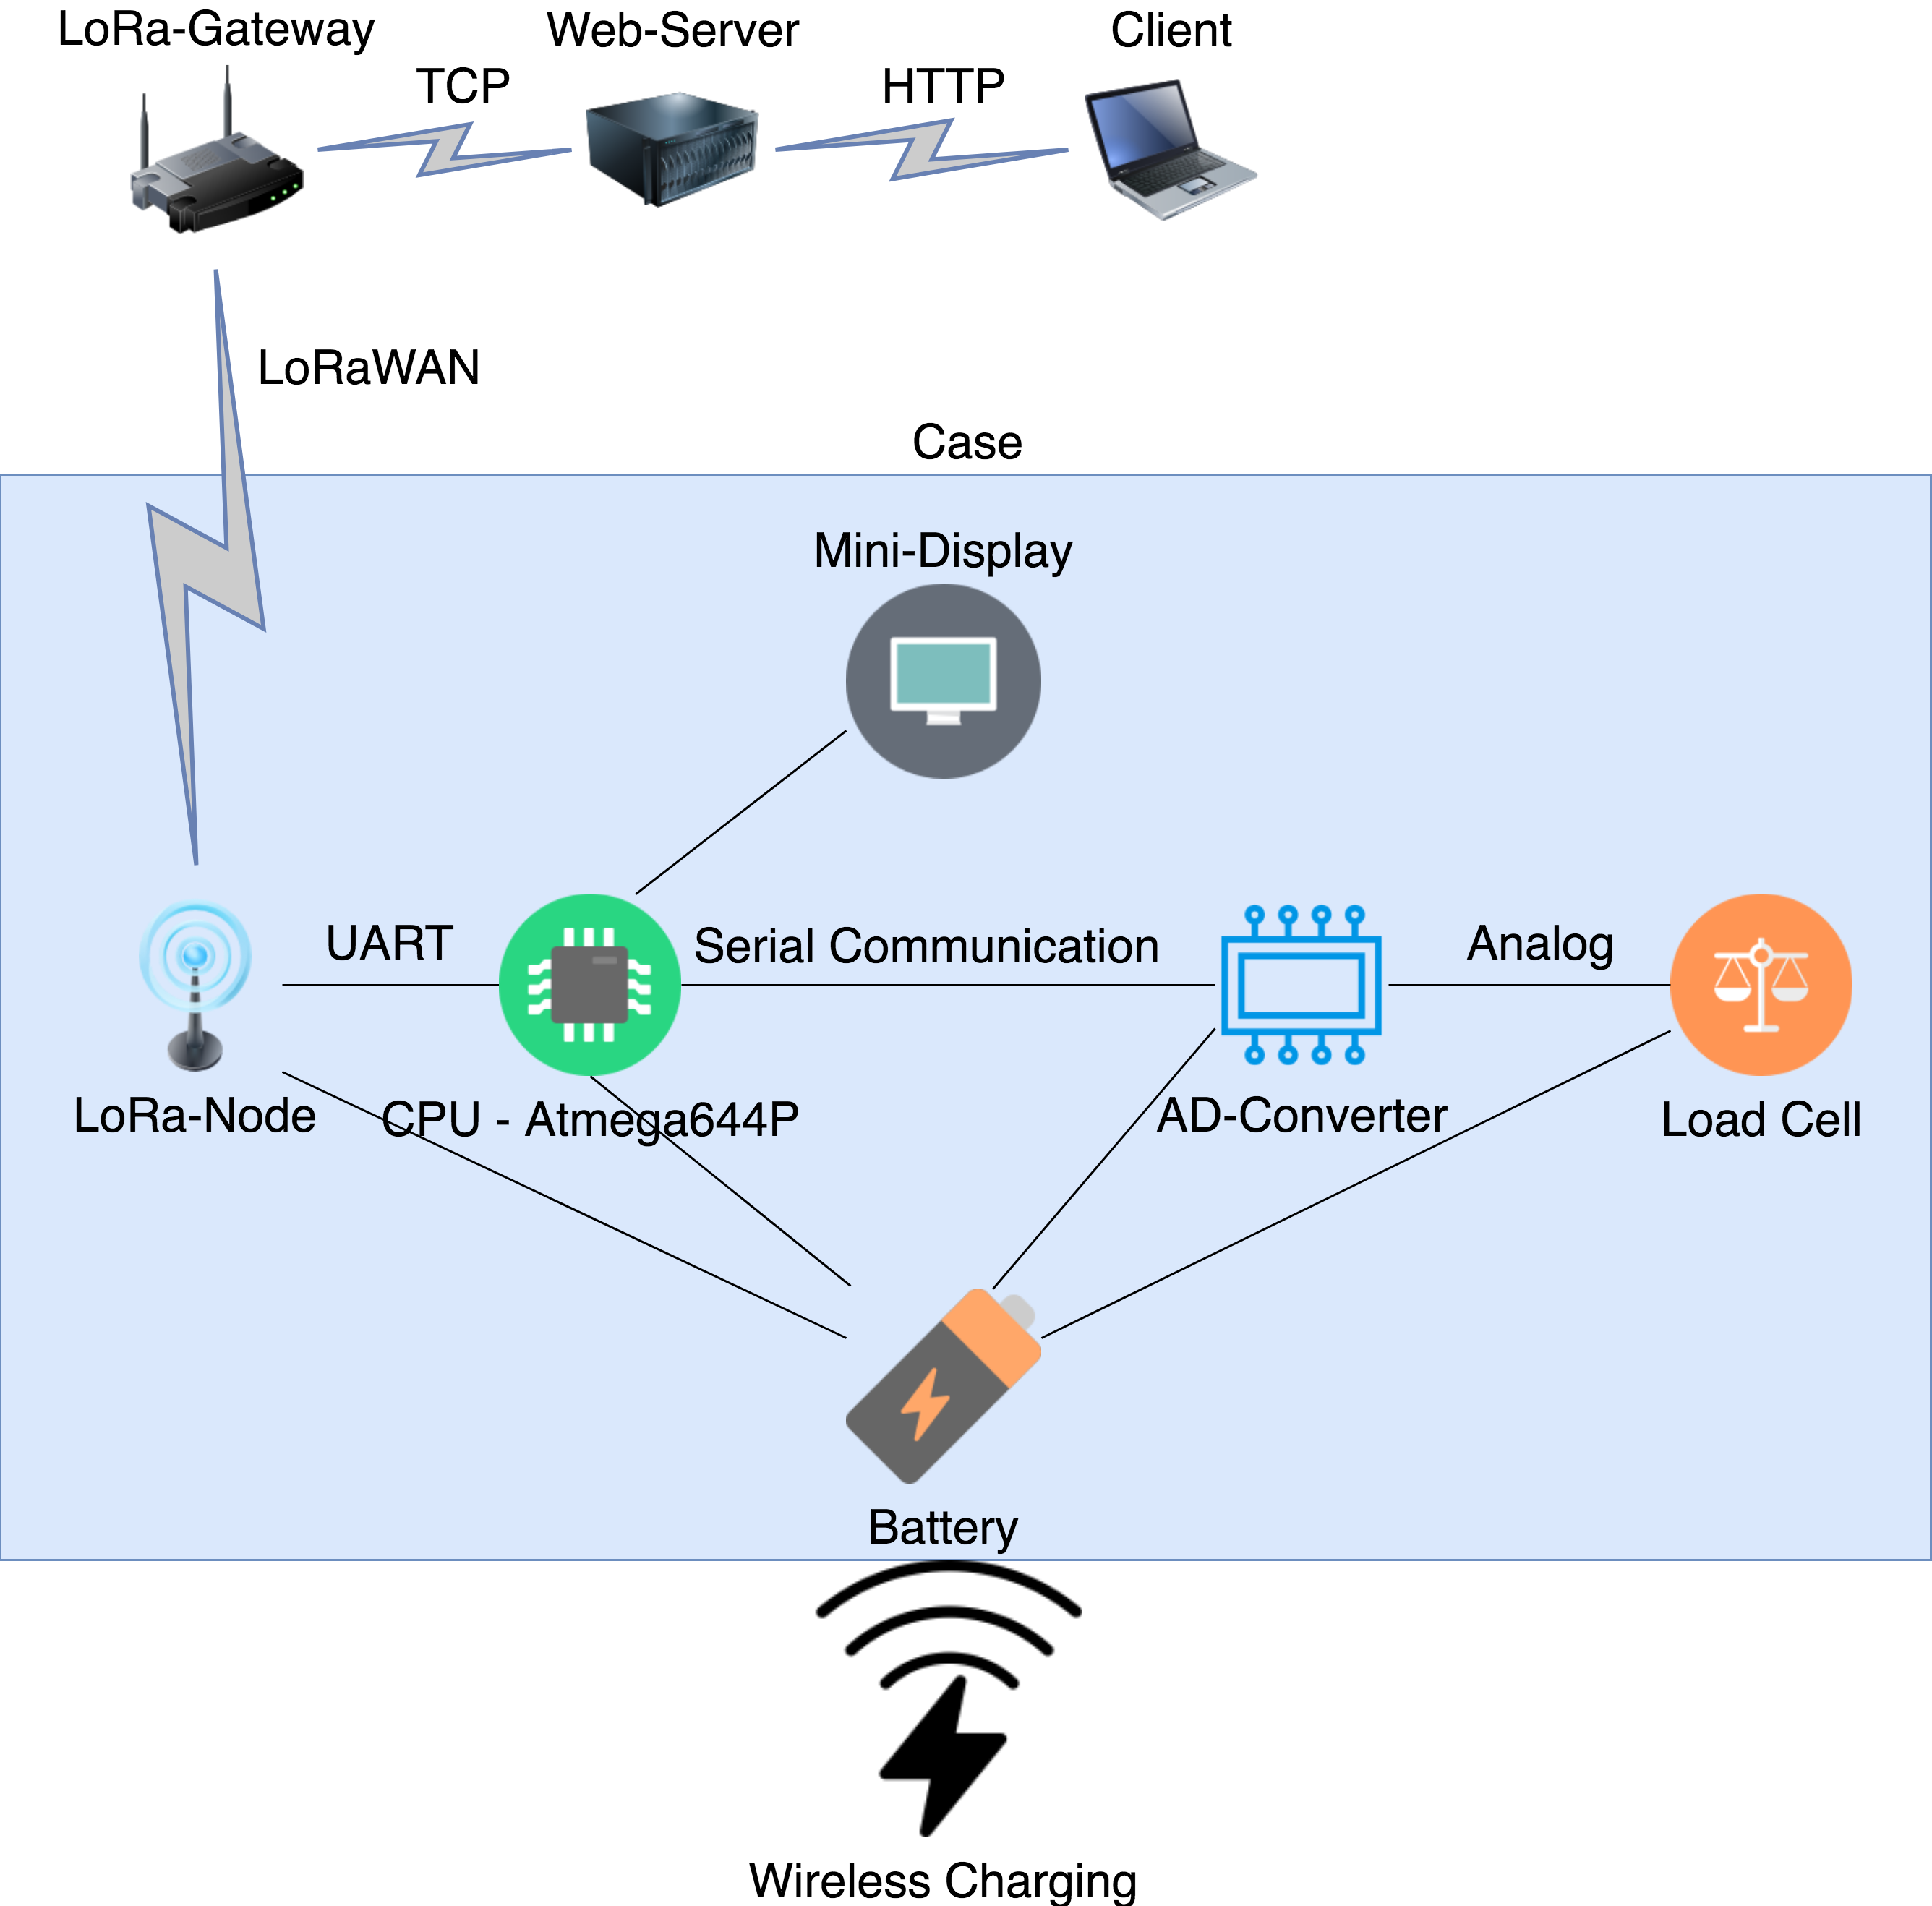
\includegraphics[width=15cm]{Bilder/komponentenmodell.png}\\
    \caption{Komponentenmodell, erstellt mit \url{https://www.draw.io/}}
    \label{fig:Komponentenmodell}
\end{figure}
\noindent
Die Herausforderung bestand dabei, die verteilten Informationen bis hin zum Client zu liefern. Da in der Gruppe die Arbeitspakete gleichzeitig abgearbeitet wurden, waren wir gezwungen für die einzelnen Testphasen Dummydaten zu erstellen, die das jeweils andere bzw. zuliefernde Modul ersetzt.
Das Gehäuse (hier 'Case') beinhaltet alle Komponenten für den Prozess des Wiegens einer Kaffee-Kanne. Der darin enthaltene LoRa-Knoten (hier: LoRa-Node) übermittelt mit Hilfe des LoRaWAN-Protokolls die jeweiligen Sensordaten mit Adresse und Zeitstempel an das LoRa-Gateway, welches alle Knoten in Empfang nimmt.

\chapter{Überblick der Bauteile}
\section{LoRa-Gateway als Empfänger der Sensordaten}
\begin{figure}[H]
    \center
    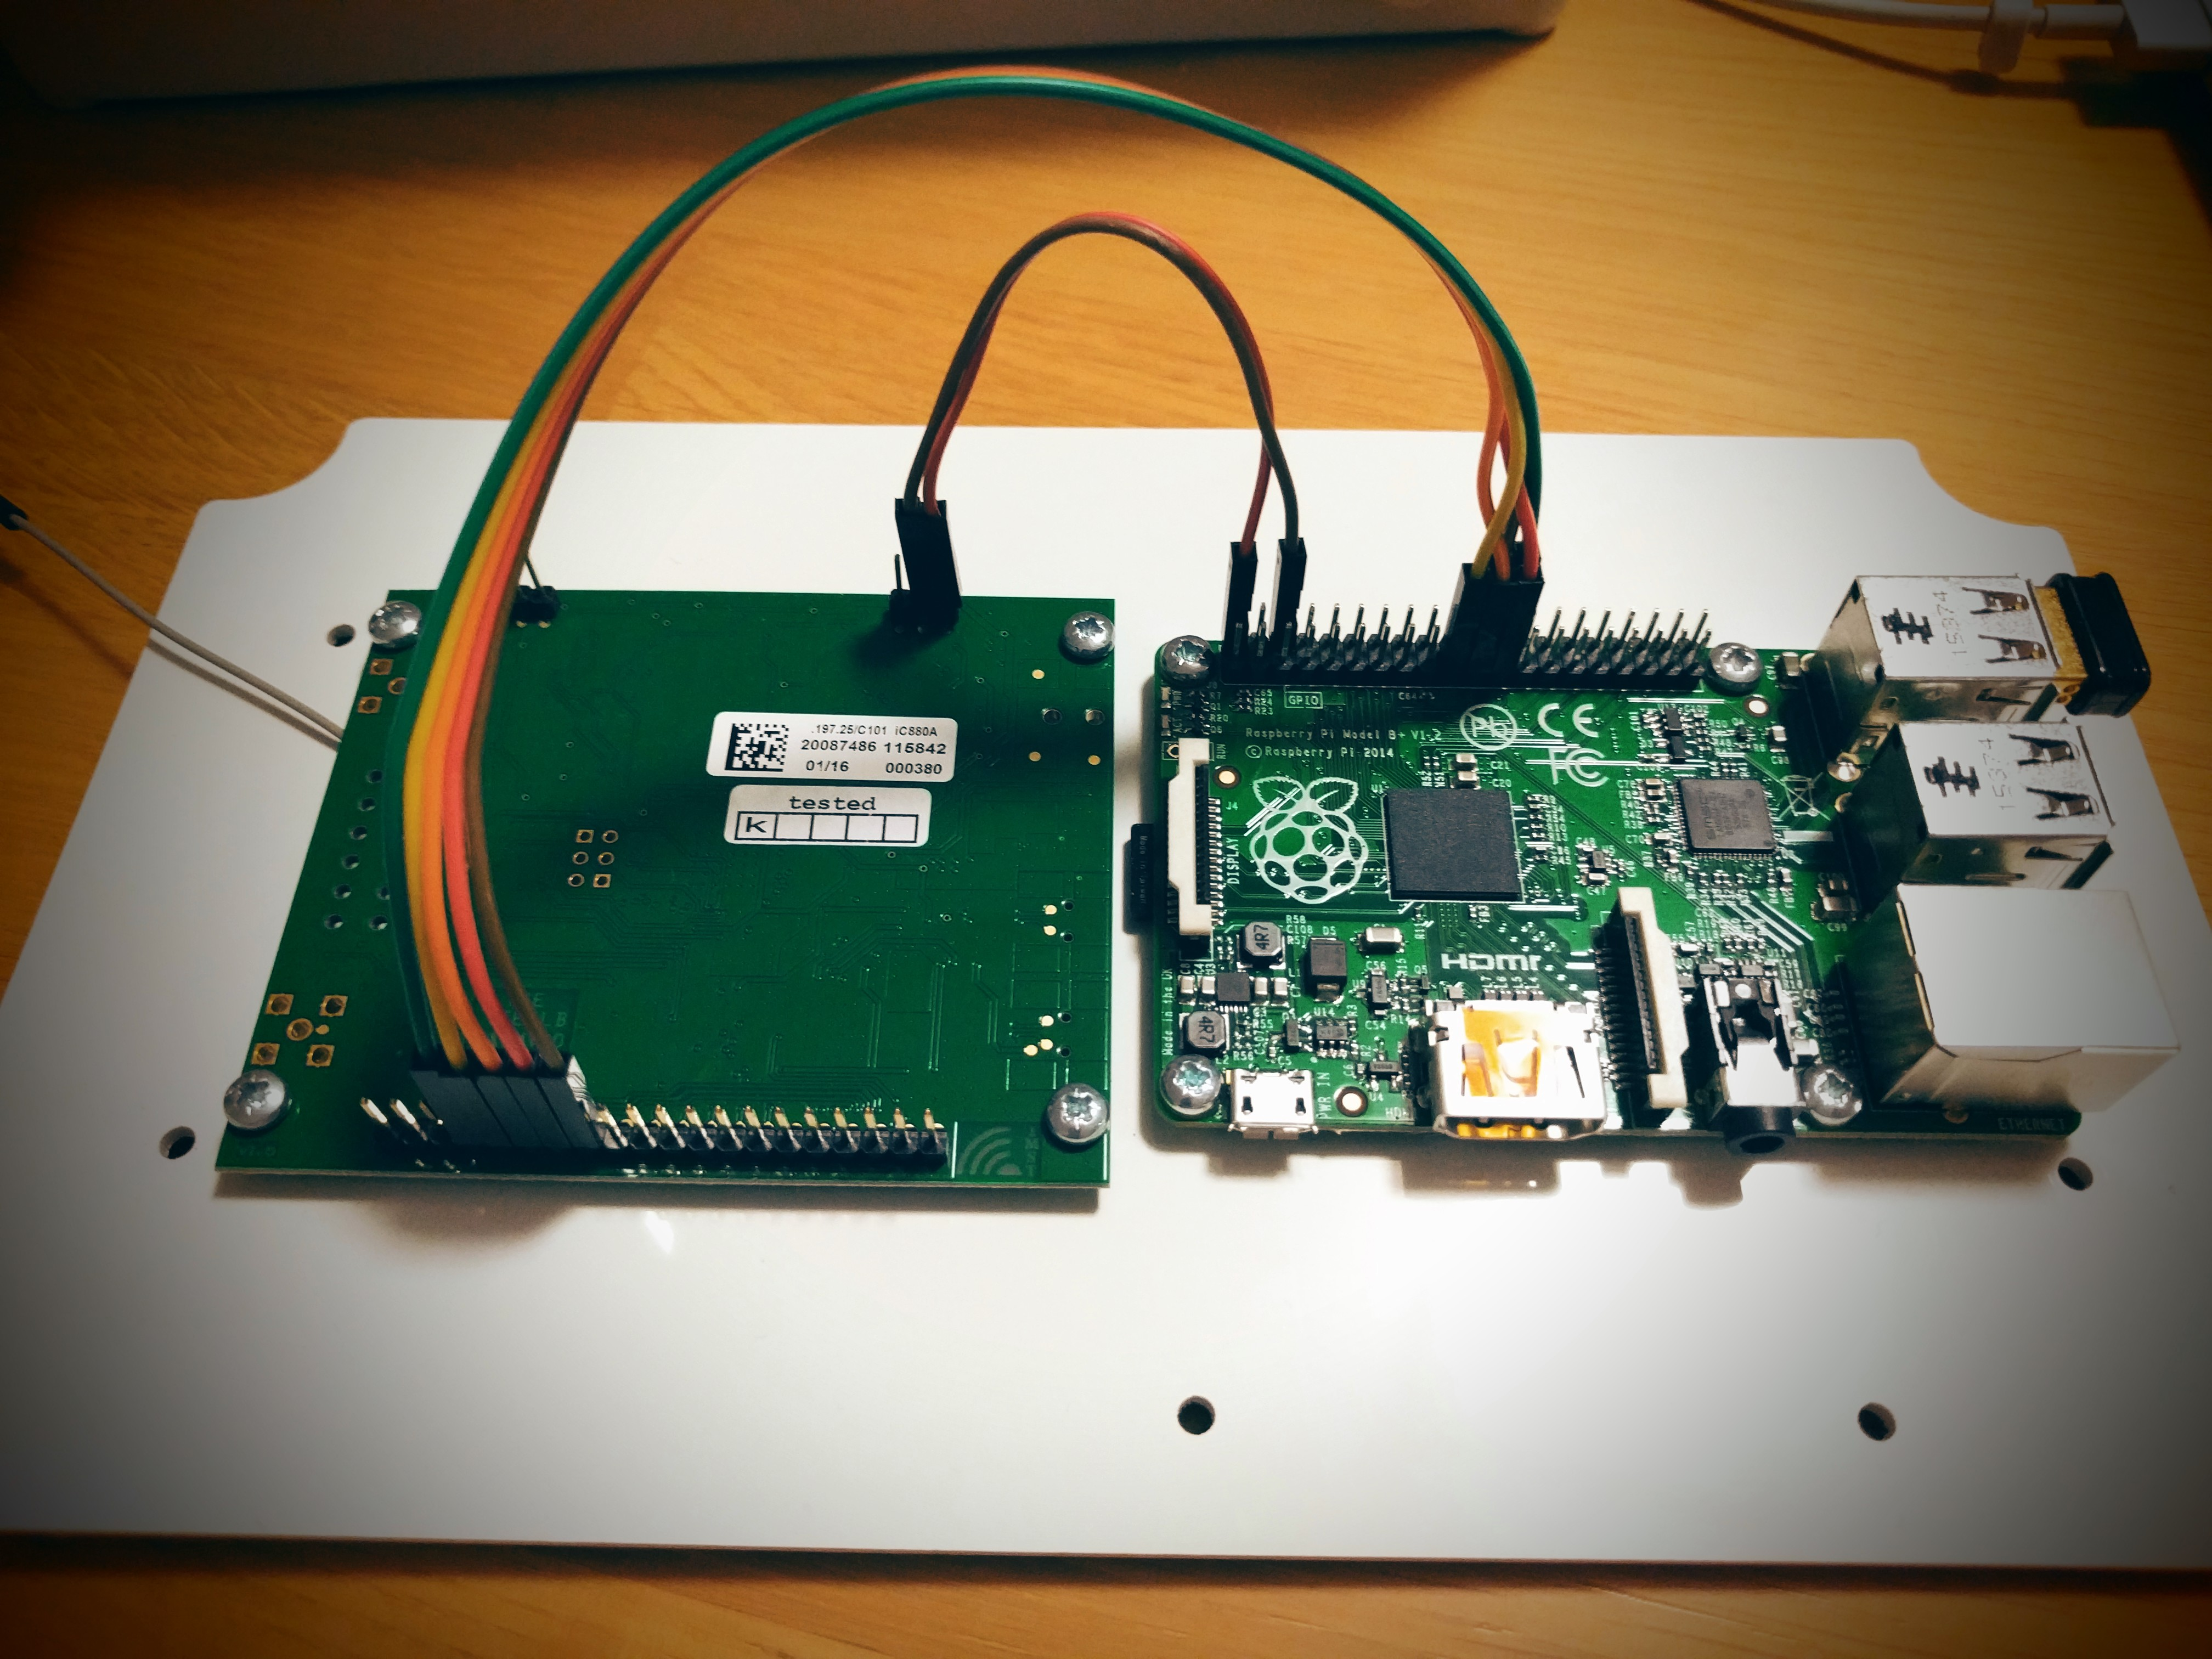
\includegraphics[width=15cm]{Bilder/mounted-boards.jpg}\\
    \caption{iC880A-SPI Concentrator Board (links) und Raspberry Pi Model 2B (rechts) bilden zusammen das Gateway, welches die Sensordaten der LoRa-Nodes empfängt und zu einem Web-Server weiterleitet.}
    \begin{flushleft}
        \quelle\url{https://raw.githubusercontent.com/ttn-zh/ic880a-gateway/spi/images/mounted-boards.jpg}
    \end{flushleft}
    \label{fig:UeberblickDerBauteile}
\end{figure}
\newpage
\section{Wägezelle als Gewichtssensor}
\begin{figure}[H]
    \center
    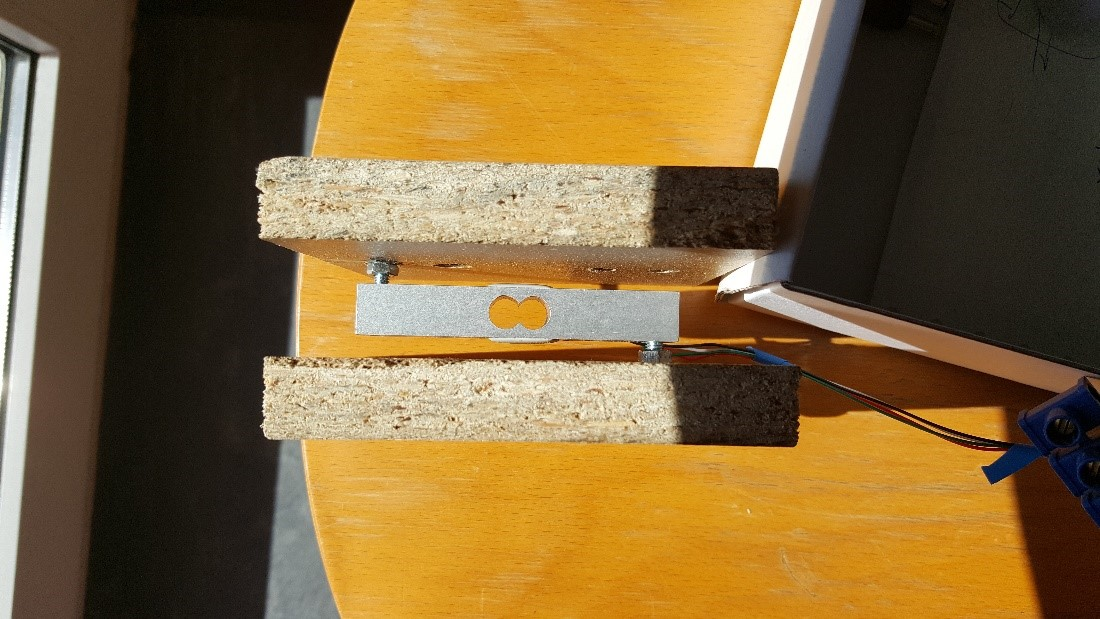
\includegraphics[width=15cm]{Bilder/waegezelle.jpg}\\
    \caption{Eine 20Kg Wägezelle wird für die Gewichtsmessung zwischen zwei Spanholzplatten befestigt. Während der Gewichtsmessung liegt die untere Spanholzplatte am Boden an und auf der oberen Spanholzplatte wird das zu messene Gewicht aufgelegt.}
    \label{fig:Waegezelle}
\end{figure}
\newpage
\section{ADC zur Wandlung und Verstärkung von Signalen}
\begin{figure}[H]
    \center
    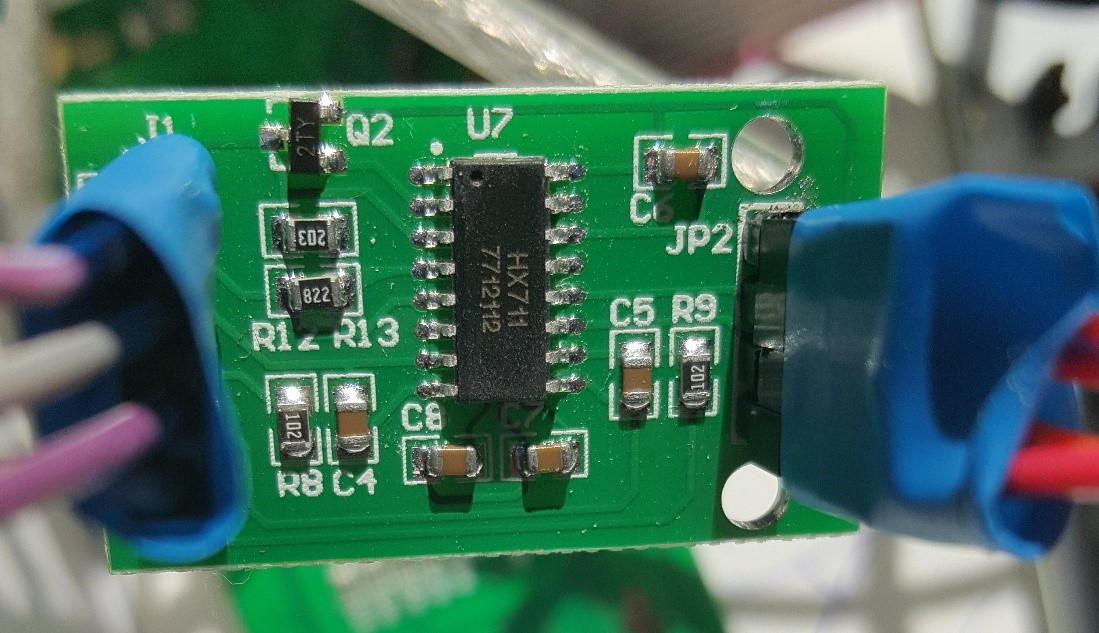
\includegraphics[width=14cm]{Bilder/gewichtssensor.jpg}\\
    \caption{Ein HX711 24-Bit ADC zur Analog-Digital-Wandlung und Verstärkung des Signals zwischen Gewichtssensor und Mikrocontroller}
    \label{fig:Gewichtssensor}
\end{figure}
\newpage
\section{LoRa-Node als Sender der Sensordaten}
\begin{figure}[H]
    \center
    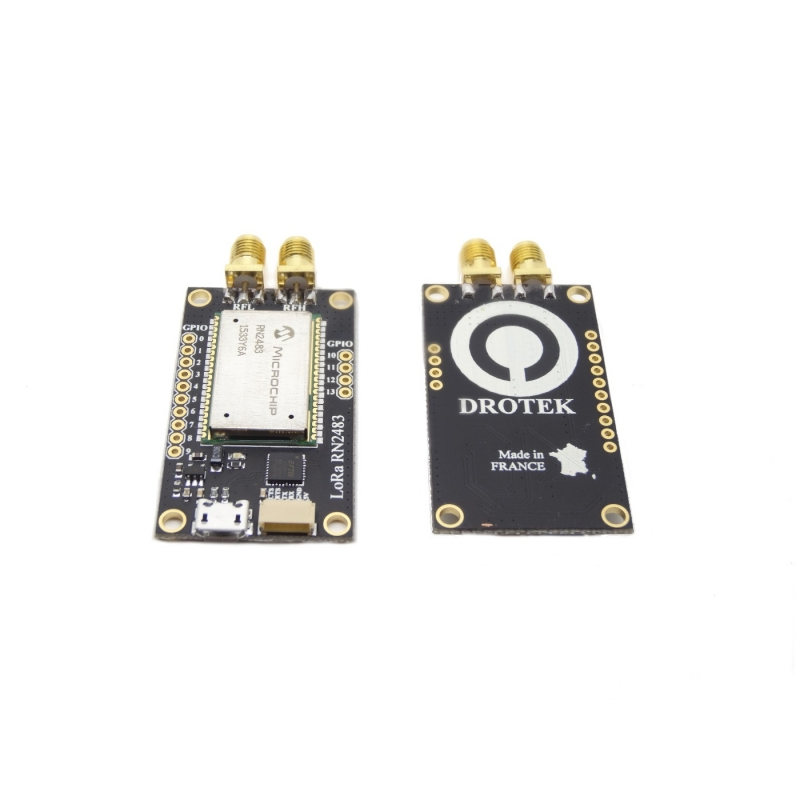
\includegraphics[width=14cm]{Bilder/lora-node.jpg}\\
    \caption{Data Link LoRa RN2483 als LoRa-Node, das zum Senden der Sensordaten über das LoRaWAN-Protokoll verwendet wird.}
    \begin{flushleft}
        \quelle\url{https://drotek.com/shop/2643-thickbox_default/data-link-lora-rn2483.jpg}
    \end{flushleft}
    \label{fig:Lora-Node}
\end{figure}

\chapter{Gewichtsmessung mit einer Wägezelle}
Um die Kaffeekanne und deren Füllstand zu messen, entschied sich das Team nach Sondierung mehrerer Alternativen (Drucksensoren, visuelle Sensoren) für die Gewichtsmessung. Dazu soll die Technik einer Wägezelle zum Einsatz kommen. In Personen- oder Küchenwaagen sind sie in millionenfacher Ausführung verbaut, was beweist, dass sie valide genutzt werden können. Weitere Alternativen, nicht nur zum Einsatz, sondern auch in der Bauform sind in Kapitel \ref{sec:use-cases-straight-bar-waegezellen} ff. zu finden.
\section{Funktionsweise der Wägezelle}
Wägezellen sind Sensoren, die das Gewicht über Verformung ihres Materials mit Hilfe von Dehnungsmessstreifen messen können. Es sind vier Dehnungsmesstreifen, wie im Bild unten zu sehen, an der Wägezelle angebracht.
\begin{figure}[H]
    \center
    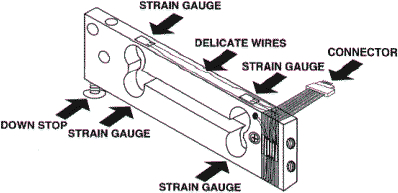
\includegraphics[width=15cm]{Bilder/waegezelle-aufbaubeschreibung.jpg}\\
    \caption{Aufbaubeschreibung einer Wägezelle}
    \begin{flushleft} \quelle\url{https://learn.sparkfun.com/tutorials/getting-started-with-load-cells} \end{flushleft}
\end{figure}
\noindent
Bei Auflage von Gewicht bzw. Verformung der Wägezelle messen zwei Dehnmessstreifen die Kompression und die anderen zwei die Spannung. Bei Kompression des Dehnmessstreifens werden die Leiter dicker (höherer Leiterquerschnitt) und kürzer (geringere Leiterlänge). Laut der Formel für den Leiterwiderstand 
\begin{equation}
    R=p \cdot \frac{I}{A}
\end{equation}
\begin{equation}
    Leiterwiderstand=\textit{spezifischer Widerstand} \cdot \frac{\textit{Leiterlänge}}{Leiterquerschnitt}
\end{equation}
verringert sich der Widerstand des Dehnungsmessstreifens. Bei Spannung des Dehnmessstreifens werden die Leiter dünner und länger, somit erhöht sich auch der Widerstand des Dehnungsmessstreifens. 
\newpage
\begin{figure}[H]
    \center
    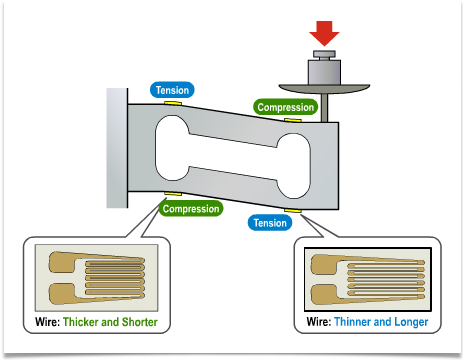
\includegraphics[width=15cm]{Bilder/waegezelle-funktionsweise.png}\\
    \caption{Funktionsweise einer Wägezelle bei Gewichtsmessung }
    \begin{flushleft} \quelle\url{https://learn.sparkfun.com/tutorials/getting-started-with-load-cells} \end{flushleft}
\end{figure}
\noindent
Um die Widerstandsveränderungen der Dehnungsmessstreifen messen zu können, sind die Dehnungsmessstreifen innerhalb der Wägezelle in einer Wheatstone-Brücken-Formation geschalten.
Die Wägezelle wird mit vier Dehnungsmessstreifen ausgestattet. Diese sind in ihrer Form, in der Länge und der geometrischen Anordnung genau gleich. [vgl. Al-Mutlaq, Sarah: Getting Started with Load Cells, URL: \url{https://learn.sparkfun.com/tutorials/getting-started-with-load-cells}, (Stand 06.07.2018)]

\newpage

\begin{figure}[H]
    \center
    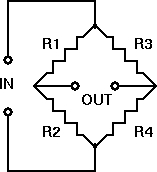
\includegraphics[width=5cm]{Bilder/waegezelle-verschaltung.jpg}\\
    \caption{Verschaltung der Dehnmessstreifen, wobei die Widerstände R1-R4 die jeweiligen Dehnmessstreifen darstellen.}
    \begin{flushleft} \quelle\url{https://learn.sparkfun.com/tutorials/getting-started-with-load-cells} \end{flushleft}
    \label{fig:waegezelle-verschaltung}
\end{figure}
\noindent
Wenn für die Verschaltung der Dehnungsmessstreifen gilt: 
\begin{equation}
    \frac{R1}{R2}=\frac{R3}{R4}
\end{equation}
dann misst man 0V an Out (siehe Abb. \ref{fig:waegezelle-verschaltung}). Falls sich ein Widerstand verändern sollte, zum Beispiel durch Verformung eines Dehnmessstreifens (d.h. stellt man eine Kaffeekanne auf die Wägezelle), lässt sich eine Spannung an Out laut dieser Formel messen: \\
%Formel:
\begin{equation}
    Vout=(\frac{R3}{(R3+R4)}-\frac{R2}{(R1+R2)}) \cdot Vin
\end{equation}

\noindent
In Abbildung \ref{fig:waegezelle-full} sind die verschalteten Dehnungsmessstreifen unter Wirkungseinfluss zu sehen und damit die Auslenkung der jeweiligen Streifen.

\begin{figure}[H]
    \center
    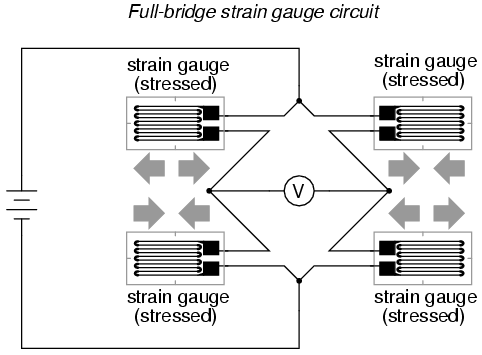
\includegraphics[width=9cm]{Bilder/waegezelle-full.png}\\
    \caption{Verschaltung der Dehnmessstreifen mit Spannungsmessung}
    \begin{flushleft} \quelle\url{https://learn.sparkfun.com/tutorials/getting-started-with-load-cells} \end{flushleft}
    \label{fig:waegezelle-full}
\end{figure}
\noindent
Die nun an \textit{Out} (siehe Abb. \ref{fig:waegezelle-verschaltung}) oder an \textit{V} (siehe Abb. \ref{fig:waegezelle-full}) gemessene analoge Spannung ist sehr klein. Für eine Abbildung der analogen Spannung auf digitale Werte ist ein Analog-Digital-Wandler (AD-Wandler) nötig, welcher nicht nur die Signale verstärkt, sondern auch die digitalen Werte repräsentiert. Der zu unserer Wägezelle angebotene integrierte Schaltkreis (englisch \textit{integrated circuit}, kurz IC, siehe Wikipedia \url{https://de.wikipedia.org/wiki/Integrierter_Schaltkreis}) war der HX711, der die gemessenen Spannungen bis zu 128-fach verstärkt und mit einer Präzision von 24 Bit [0 bis 16777217] wandelt.
\newpage


\section{Versuchsaufbau zur Gewichtsmessung}
Die Wägezelle wurde an zwei gegenüberliegenden Punkten an zwei Holzplatten geschraubt, damit sich das Gewicht auf alle Dehnungsmesstreifen auswirkt.\\
\begin{figure}[H]
    \center
    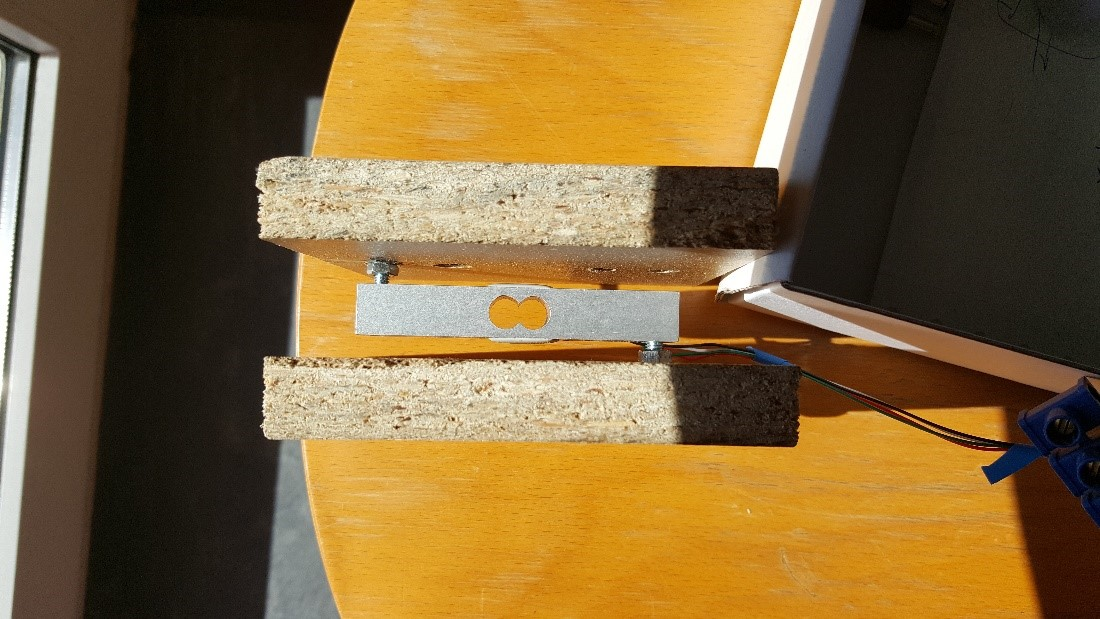
\includegraphics[width=15cm]{Bilder/waegezelle.jpg}\\
    \caption{20Kg Wägezelle zwischen zwei Spanholzplatten befestigt}
\end{figure}
Die Wägezelle wurde wie folgt an das HX711-Modul angeschlossen: 
\begin{itemize}
    \item Rot an E+ (Excitation+/Vin+) 
    \item Schwarz an E- (Excitation-/Vin-) 
    \item Weiß an A+ (Output+/Vout+) 
    \item Grün an A- (Output-/Vout-) 
\end{itemize}

\newpage
\noindent
Veranschaulichung der Verdrahtung (Achtung! Gelbe Verbindung ist bei uns weiß):\\
\begin{figure}[H]
    \center
    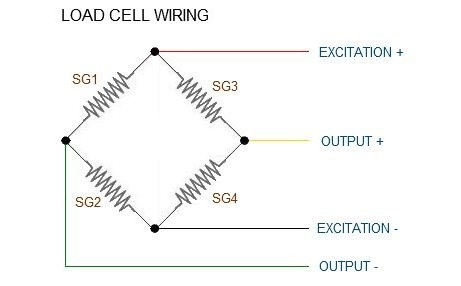
\includegraphics[width=9cm]{Bilder/waegezelle-verdrahtung.jpg}\\
    \caption{Verdrahtung der Wägezelle }
    \begin{flushleft} \quelle\url{https://learn.sparkfun.com/tutorials/load-cell-amplifier-hx711-breakout-hookup-guide} \end{flushleft}
\end{figure}
\noindent
Die A-Anschlüsse und B-Anschlüsse des HX711 (siehe Abbildung \ref{fig:waegezelle-adc} HX711 linke Kontaktseite) sind für verschiedene Verstärkungskanäle. Der A-Kanal hat einen programmierbaren Verstärkungsfaktor von 128 oder 64 und der B-Kanal hat einen festen Verstärkungsfaktor von 32.
\newpage
Die rechte Seite des HX711 wird wie folgt angeschlossen: 
\begin{itemize}
    \item GND an Ground 
    \item VCC an Versorgungsspannung in unserem Fall 5V 
    \item SCK an PD5 unseres Microcontrollers/ATmega644PA 
    \item DT (Data) an PD6 unseres Microcontrollers/ATmega644PA 
\end{itemize}
\begin{figure}[H]
    \center
    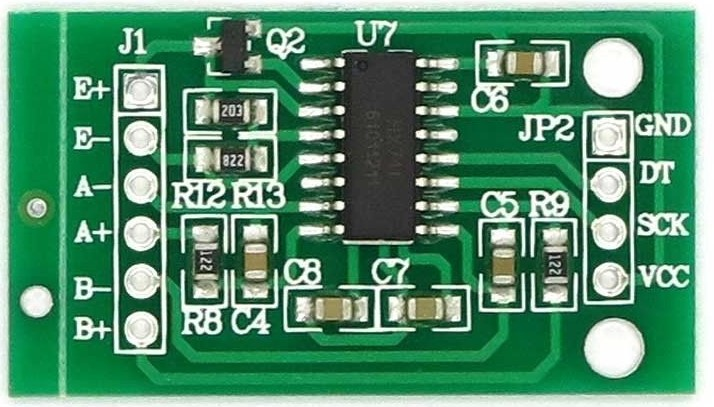
\includegraphics[width=9cm]{Bilder/waegezelle-adc.jpg}\\
    \caption{HX711 ADC-Wandler, Ansicht auf Bauteil}
    \quelle\url{https://tinyurl.com/y8grwwdb}
    \label{fig:waegezelle-adc}
\end{figure}
\section{Programmlogik unseres Microchips}
Nach dem Aufbau unseres Systems geht es nun an die Gewichtsmessung. Das Programm zur Gewichtsmessung mittels dem HX711 basiert auf \textit{getsiddd's HX711 AVR Bibliothek} (\url{https://github.com/getsiddd/HX711}).\\ 
\\
Die wichtigsten Erweiterungen von uns sind:
\begin{itemize}
    \item die Möglichkeit, negative Gewichtsveränderungen wahrnehmen zu können, siehe Funktion weightStuff() in RN2483.c, Zeile 246-254
    \item auf Tastendruck eine Tar-Funktion auszuführen, siehe Funktion weightStuff() in RN2483.c, Zeile 312-316
    \item Gewichts-Sende-Algorithmus in Verbindung mit dem LoRa-Modul, siehe Funktion ISR(TIMER0\_COMPA\_vect) in RN2483.c, Zeile 146-194
\end{itemize}
\subsection{Vereinfachte Funktionsweise für momentane Gewichtsmessung}
\noindent
Nachdem die Bibliothek für den Baustein HX711 angepasst ist, also das Gewicht gemessen und versendet werden kann, geht es darum einen visualisierbaren Wert zu erhalten. Jedoch sind nicht alle Wägezellen perfekt gleich und ohne Rücksicht auf diese Imperfektionen würde jede Wägezelle einen anderen Messwert ergeben. 
Um dieses Problem zu lösen, ist eine Kalibrationsvariable im Code implementiert. In unserem Fall, ist die Kalibrationsvariable ein fest codiertert Parameter, der durch ``Trial und Error'' ertestet wird, indem wir ein bekanntes Gewicht auf die Wägezelle legen und den Kalibrationswert in Richtung des gesuchten Gewichtes anpassen. Mit dem Ergebnis aus der Kalibrierung ist die Gewichtsmessung möglich.\\
\\
Dazu ein kurzer Programmablauf der Funktionsweise:
\begin{itemize}
    \item das Gewicht wird zunächst gelesen (Bsp.: 8563)
    \item das ge'tar'te Gewicht wird davon abgezogen ($8563 - 6546 = 2017$)
    \item anschließend wird durch das Ergebnis der Kalibrierung geteilt: ($2017 / 2000 = 1,0085$)
    \item um am Ende einen lesbaren Kilogrammwert zu bekommen: 1,0085 Kg
\end{itemize}
\subsection{Algorithmus für Rausch- und Driftunterdrückung}
Das Differenzgewicht von der letzten und der momentanen Gewichtsmessung wird mit einer vorher gewählten Veränderungsrate verglichen. Wenn das Differenzgewicht höher als die gewählte Veränderungsrate ist, wird der momentan gemessene Wert verwendet und angezeigt, im anderen Fall wird der Wert verworfen, weil er vermutlich durch Rauschen oder Drift verursacht wurde.\\
Der Veränderungswert gibt auch die kleinstmögliche messbare Veränderung an. Am Beispiel unseres Projektes könnte bei einem Veränderungswert von ca. 5g, jemand mit einem Strohhalm Flüssigkeit aus dem Behältnis saugen, ohne dass das Programm die Gewichtsveränderung wahrnimmt.
\subsection{Algorithmus für Gewichtssendung mit dem LoRa-Modul}
Die gemessenen Gewichtsdaten müssen nun an die Sammelstelle (den Gateway) gesendet werden. Der Sendevorgang basiert auf dem LoRa-Protokoll, welches vom LoRa-Modul in Empfang und in regelmäßigen Abständen zum LoRa-Gateway gesendet wird (vgl. \ref{fig:Komponentenmodell} Komponentenmodell). Mit Hilfe eines Interrupts, wird jede Sekunde eine Gewichtsmessung durchgeführt. Beim Ablauf des Sendeintervalls (in unserem Projekt momentan eingestellt auf fünfzehn Sekunden), wird in der Menge der Gewichtsmessungen (in unserem Fall fünfzehn Messungen, jede Sekunde eine), nach den letzten fünf Gewichtsmessungen gesucht, die den gleichen Wert haben. Wenn die Messungen diese Bedingung nicht erfüllen, wird kein Wert gesendet.

\section{Demonstration der Gewichtsmessung}
Hier eine Demo zur Gewichtsmessung, die wir auch in der Zwischenpräsentation gezeigt haben:\\
\url{https://streamable.com/ycxf3}\\
Alternativ: \url{https://www.youtube.com/watch?v=2tk0ydRsXgg}

\section{Alternative Use-Cases von “Straight bar”-Wägezellen}
\label{sec:use-cases-straight-bar-waegezellen}
Die Art, der von uns verwendeten Wägezellen, wird unter anderem in diesen Bereichen verwendet:
\begin{itemize}
    \item Küchenwaagen
    \item Industrielle Gewichtsmessung, die an einem Punkt erfolgt
    \item Personenwaagen
    \item (geeichte) Handelswaagen für Obst, Fleisch, Käse, Gemüse
\end{itemize}
\newpage
\section{Alternative Bauformen von Wägezellen}
Es gibt überhaupt viele Möglichkeiten zu wiegen. Neben den Wägezellen sind auch andere technische Lösungen möglich, auf die wir in Kapitel \ref{sec:alternative-gewichtssensoren} kurz eingehen.\\
Wägezellen gibt es in verschiedensten Bauformen. Die folgende Aufzählung zeigt die meisten davon. Einige haben wir auch auf unsere Anforderungen hin untersucht, um für unser Projekt und entpsrechende Folgeprojekte die richtigen auswählen zu können.
\subsection{Disk-Wägezellen}
Disk-Wägezellen haben eine runde Form und sind kompakter gebaut.\\
Mögliche Einsatzgebiete sind:
\begin{itemize}
    \item Industrie bei sehr großen Gewichtsmessungen 1 - 50 Tonnen, verteilte Aufnahme der Gewichtseinwirkung
    \item Umgebungen mit wenig Platz, da sehr platzsparend einsetzbar, jedoch mit sehr hoher Ungenauigkeit. In diesem Fall liegt die Nicht-Widerholpräzision bei über 0,5\%
\end{itemize}

\begin{figure}[H]
    \center
    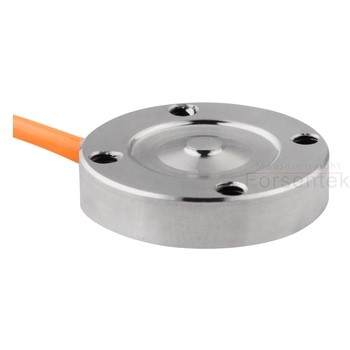
\includegraphics[width=4cm]{Bilder/waegezelle-disk.jpg}\\
    \caption{Disk-Wägezelle}
    \begin{center} \quelle\url{http://www.forsentek.com/prodetail_13.html} \end{center}
\end{figure}
\newpage
\subsection{Wägesensoren}
Wägesensoren besitzen nur einen Dehnmessstreifen anstatt herkömmliche, die vier besitzen. Man kann vier Wägesensoren in einer Wheatstone-Bridge-Formation zusammen schalten und wie eine Straight-Bar-Wägezelle betreiben. Dabei kann man die einzelnen Wägesensoren auf einer größeren Fläche betreiben und sie als Personenwaage, Fahrzeugwaage oder allgemein als Waage für große Objekte verwenden.
\begin{figure}[H]
    \center
    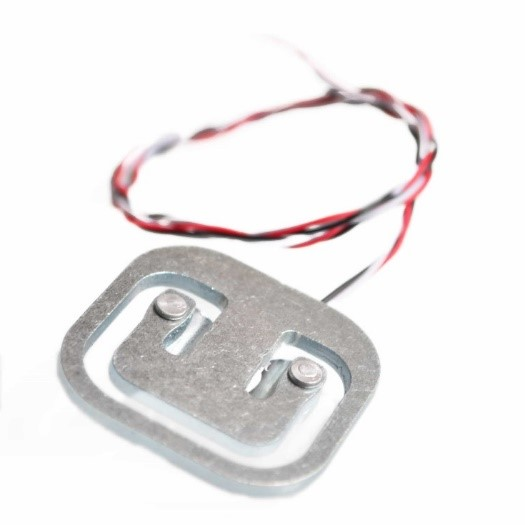
\includegraphics[width=4cm]{Bilder/waegezelle-waegesensor.jpg}\\
    \caption{Wägesensor}
    \begin{center} \quelle\url{https://www.botshop.co.za/product/load-cell-sensor-resistance-strain-50kg/} \end{center}
\end{figure}
\subsection{S-Typ-Wägezellen}
Diese Wägezellen lassen sich, dank ihrer S-Form, in Spannungs- und Kompressionsbetrieb betreiben.
\begin{figure}[H]
    \center
    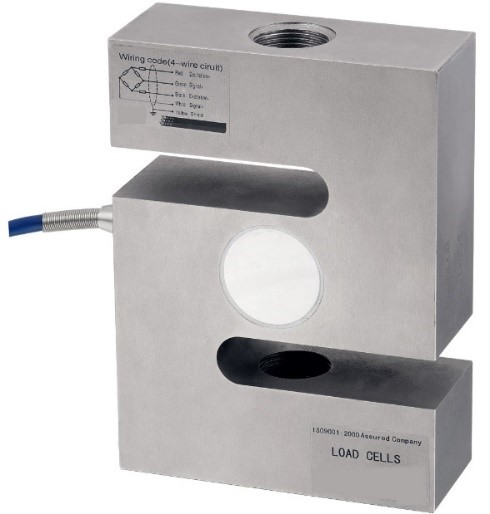
\includegraphics[width=4cm]{Bilder/waegezelle-s_typ.jpg}\\
    \caption{S-Typ-Wägezelle}
    \begin{center} \quelle\url{https://www.coventryscale.co.uk/scale-type/load-cells/tension-s-type-load-cells/s-type-load-cell/} \end{center}
\end{figure}
\newpage
\subsection{Kompressions-Wägezellen}
Diese Art von Wägezellen sind nur in Kompressionsumgebungen einsetzbar und gehören auch zur Familie der Disk-Wägezellen. Ihr Einsatzgebiet ist in hocheffizienten Industrieanwendungen, mit meist deutlich über 1Kg als Minimalgewicht.
\begin{figure}[H]
    \center
    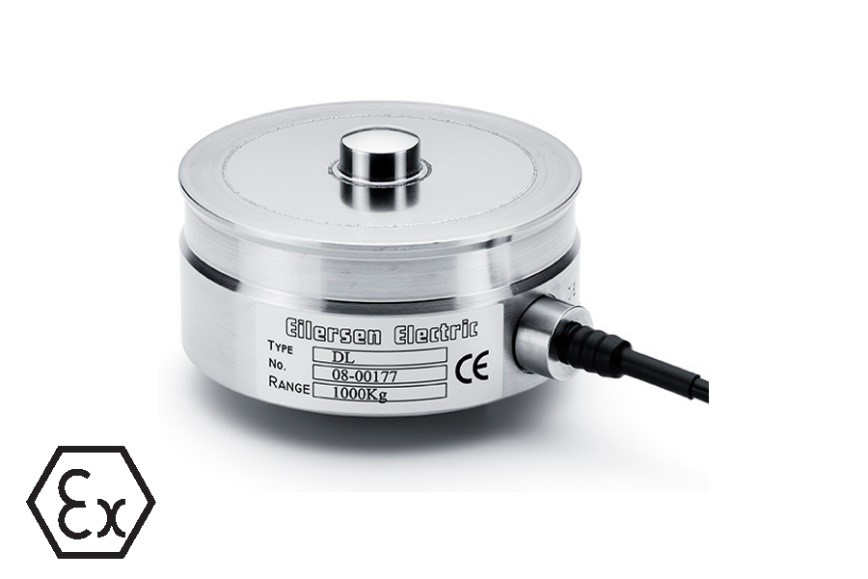
\includegraphics[width=7cm]{Bilder/waegezelle-kompression.jpg}\\
    \caption{Kompressions-Wägezelle}
    \begin{center} \quelle\url{http://www.eilersen.com/compression-load-cell/product/atex-compression-load-cell-dla/} \end{center}
\end{figure}
\newpage
\section{Alternative Gewichtssensoren}
\label{sec:alternative-gewichtssensoren}
\subsection{Force Sensitive Resistor (FSR)}
Bei Kraftzunahme beziehungsweise Kompression des Sensors verringert sich der Abstand zwischen den Sensorfolien, die voneinander mit einer speziellen Tinte getrennt sind, und somit auch ihr Widerstand. Diese Sensoren sind sehr platzsparend, aber auch ungenauer als Wägezellen, weshalb sie nicht sehr gut für die Gewichtsmessung geeignet sind.
\begin{figure}[H]
    \center
    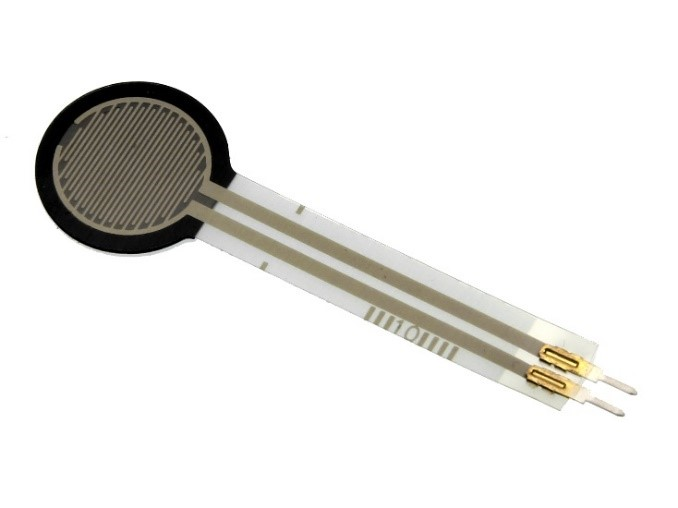
\includegraphics[width=4cm]{Bilder/waegezelle-force.jpg}\\
    \caption{Force Sensitive Resistor}
    \begin{center} \quelle\url{https://solarbotics.com/product/50803/} \end{center}
\end{figure}
\subsection{Piezoelektrischer Sensor}
Bei Krafteinwirkung produzieren diese Sensoren eine elektrische Ladung, die gemessen werden kann. Sie sind eher für dynamische Anwendungen geeignet, da Signale nur bei Kraftänderungen gemessen werden können, beziehungsweise die Ladung sehr schnell wieder gegen Null geht. Es gibt spezielle Varianten, die ihre Ladung bis zu einer Minute halten können, diese weisen jedoch einen hohen Drift auf. 
\begin{figure}[H]
    \center
    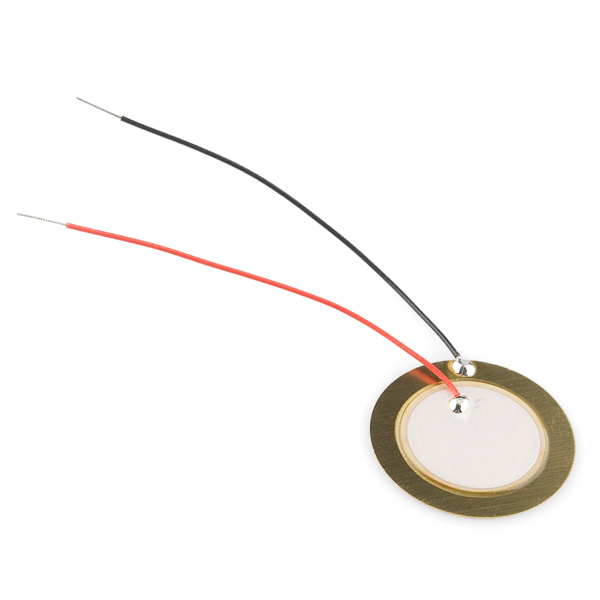
\includegraphics[width=4cm]{Bilder/waegezelle-ring.png}\\
    \caption{Piezoelektrischer Sensor}
    \begin{center} \quelle\url{https://www.sparkfun.com/products/10293} \end{center}
\end{figure}

\chapter{Drahtlose Verbindung zwischen den Komponenten mit dem LoRaWAN-Protokoll}
Nachdem wir nun zuverlässig die Sensordaten (in unserem Fall: das Gewicht und somit den Füllstand) messen und verarbeiten können, geht es in diesem Kapitel nun um das Versenden und Empfangen der Sensordaten über die drahtlose Verbindungstechnologie LoRa.
\section{Aufsetzen eines Servers (LoRa-Gateway)}
Damit wir überhaupt überprüfen können ob die Daten die wir versenden vollständig und zuverlässig ankommen, benötigen wir erstmal einen Empfänger.
Dieser Empfänger wird als LoRa-Gateway bezeichnet und hat im Prinzip die Funktion eines WLAN-Routers. Alle Clients (LoRa-Nodes) melden sich an dem Gateway an und kommunizieren mit dem Gateway. Wie der Begriff „Gateway“ schon andeutet, ist dies ein Tor, das zum Internet führt (siehe folgende Abbildung \ref{fig:lora-schaubild}).
\begin{figure}[H]
    \center
    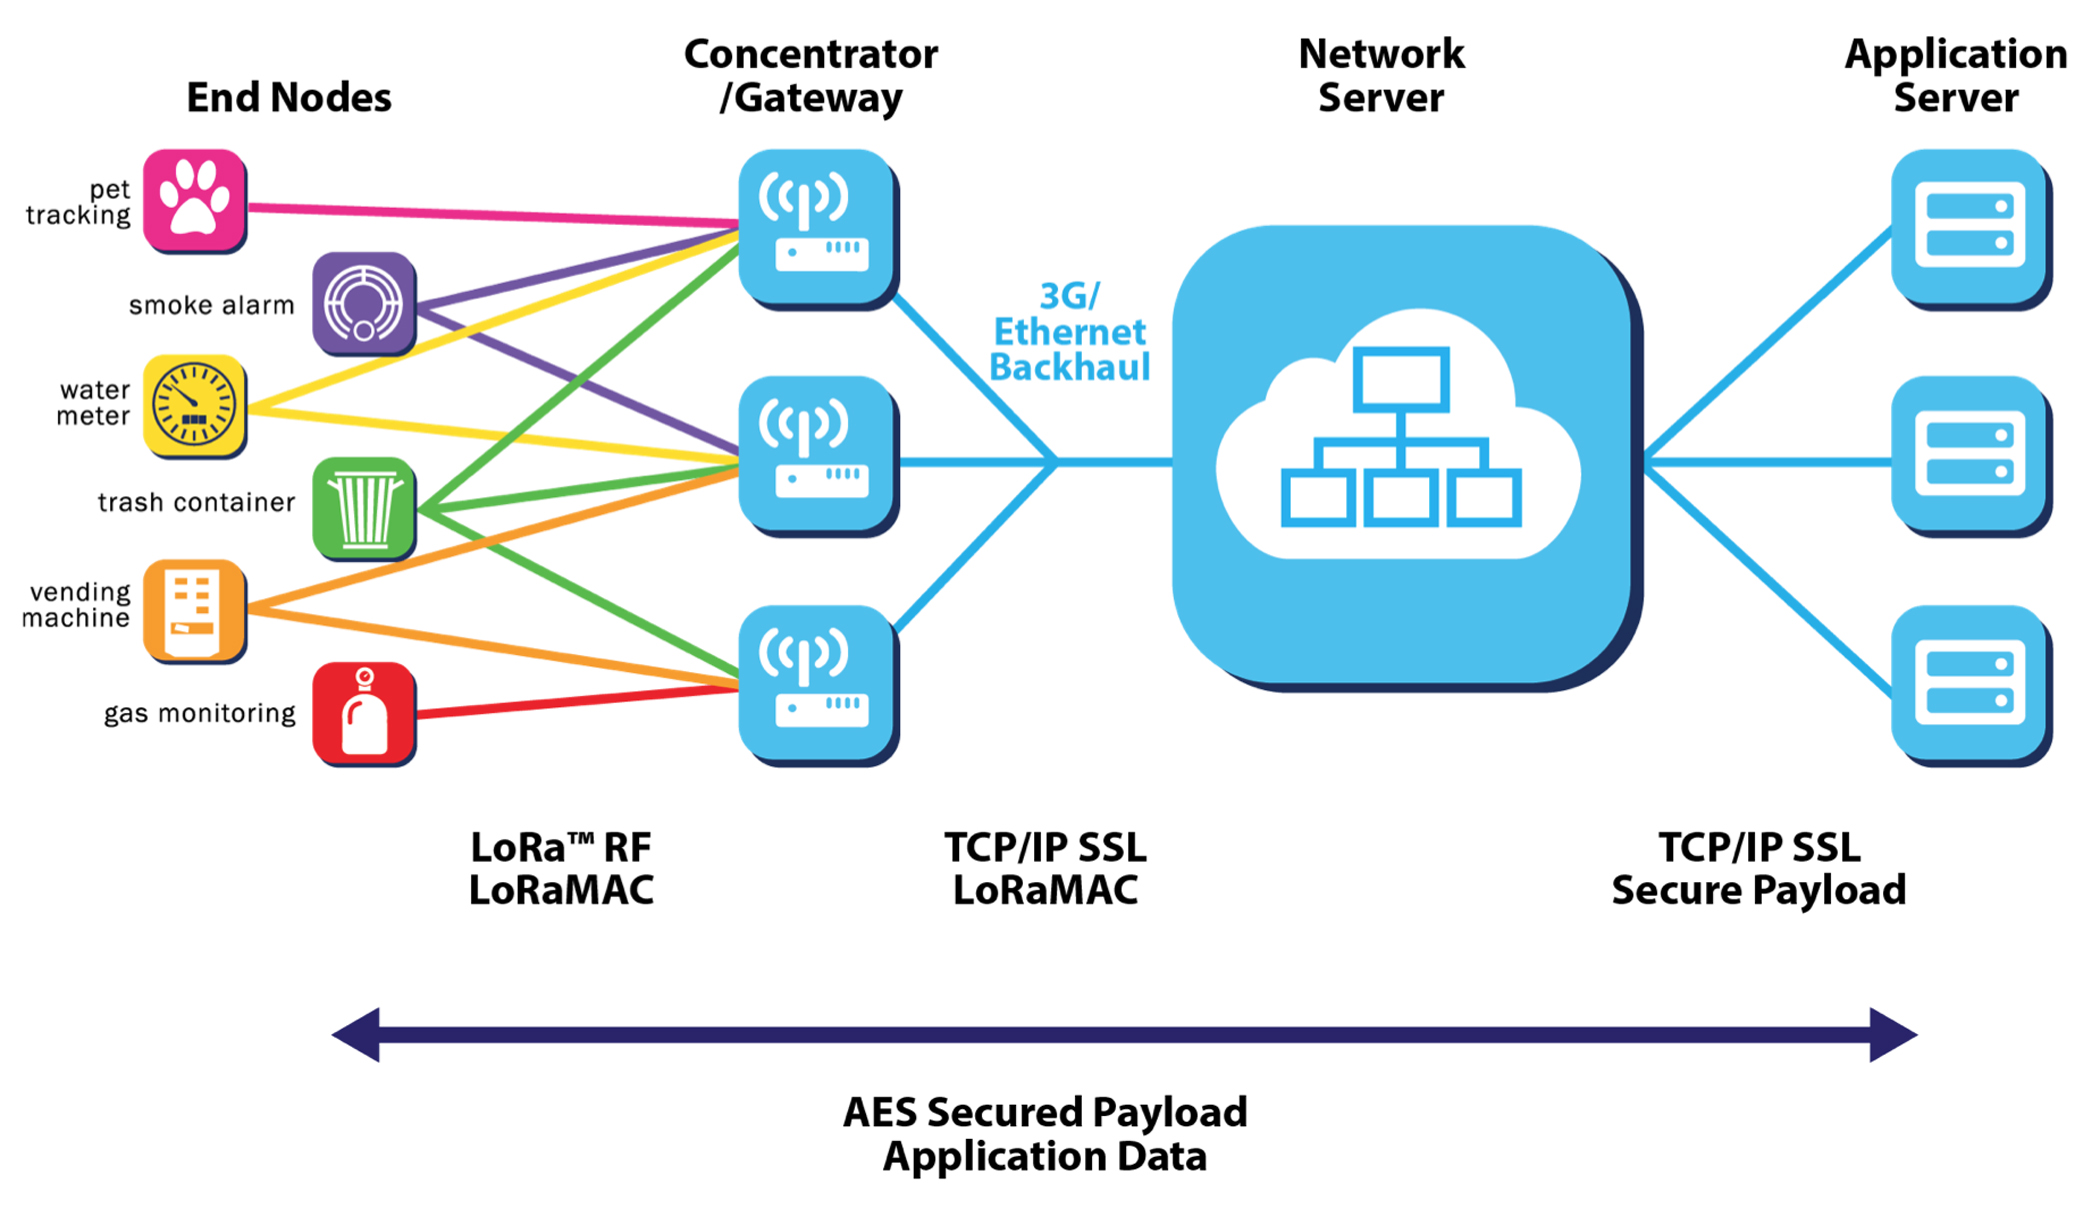
\includegraphics[width=15cm]{Bilder/lora-schaubild.jpg}\\
    \caption{Übersicht eines Beispiel-LoRa-Netzwerks}
    \begin{center} \quelle\url{http://www.mstanley.co.uk/blog/wp-content/uploads/2015/11/Enabling-world-wide-mobility-for-the-IoT-image-2.jpg} \end{center}
    \label{fig:lora-schaubild}
\end{figure}
\noindent
Realisiert wird unser Gateway durch ein „iC880A-SPI Concentrator Board“, das mit Hilfe einer Antenne mit den LoRa-Nodes Daten austauscht. Das Gateway, also das Concentrator Board, ist über ein Serial Peripheral Inface (SPI) an einen Raspberry Pi angeschlossen. Dieser Einplatinen-Computer versendet nun die Daten der LoRa-Nodes, empfangen über das Gateway, ins Internet.\\
Damit nun die gesendeten Daten nicht nur lose in der großen weiten Welt des Internets ziellos umher irren, benötigt das Gateway eine Adresse, über die Datenpakete identifiziert werden können. Doch vor der Adress-Konfiguration der Hardware, sollten die Komponenten beschafft und lokal richtig installiert werden damit sie miteinander funktionieren.\\
Auf dem Wiki der GitHub-Seite von The Things Network Zurich (\url{https://github.com/ttn-zh/ic880a-gateway/wiki}) kann man nachlesen welche Bauteile man benötigt, wie man die Pins verbinden soll, das Betriebssystem aufsetzt und anschließend das Gateway im TheThingsNetwork registriert.\\
Nachdem man die Anweisungen zum Konfigurieren befolgt hat, sollte es auf der Webseite für Gateways von TheThingsNetwork zu sehen sein (siehe folgende Abbildung \ref{fig:lora-1}).
\begin{figure}[H]
    \center
    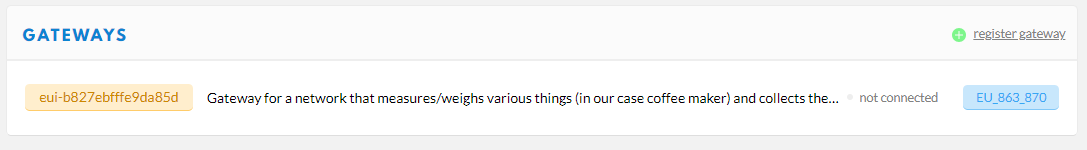
\includegraphics[width=16cm]{Bilder/lora-1.png}\\
    \caption{Übersicht der registrierten Gateways im TheThingsNetwork}
    \begin{center} \quelle\url{https://console.thethingsnetwork.org/gateways} \end{center}
    \label{fig:lora-1}
\end{figure}
\newpage
\section{Erstellen einer LoRa-Applikation zum Abrufen der Daten}
Nachdem unser Gateway nun empfangsbereit ist könnten wir eigentlich schon ein LoRa-Node in Betrieb setzen um Daten an den Gateway zu senden.
Da diese Daten aber verschlüsselt sind, müssen wir aber erstmal eine Applikation erstellen um lesbare Daten zu erhalten und sie zu einem Sender zuordnen zu können.
Eine Applikation können wir in der Konsole von TheThingsNetwork erstellen (siehe folgende Abbildungen \ref{fig:lora-2} und \ref{fig:lora-3}).
\begin{figure}[H]
    \center
    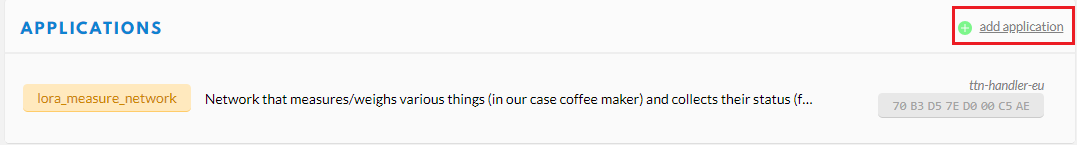
\includegraphics[width=16cm]{Bilder/lora-2.png}\\
    \caption{Übersicht der erstellten Applikationen im TheThingsNetwork}
    \begin{center} \quelle\url{https://console.thethingsnetwork.org/applications} \end{center}
    \label{fig:lora-2}
\end{figure}
\begin{figure}[H]
    \center
    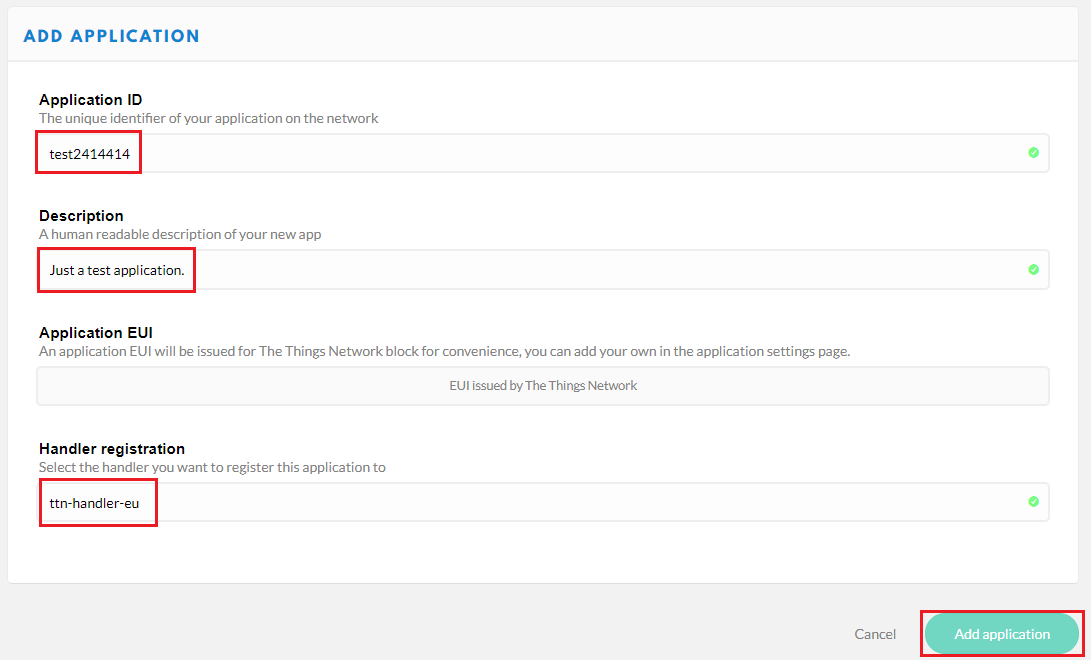
\includegraphics[width=16cm]{Bilder/lora-3.png}\\
    \caption{Formular zur Erstellung einer Applikation}
    \begin{center} \quelle\url{https://console.thethingsnetwork.org/applications} \end{center}
    \label{fig:lora-3}
\end{figure}
\newpage
\paragraph{Application ID:} Muss einzigartig und eindeutig sein.
\paragraph{Description:} Eine kurze, aber aussagekräftige Beschreibung der Applikation.
\paragraph{Handler registration:} Wurde passend zum Standort gewählt.\\
\\
Nachdem man nun eine Applikation erstellt hat, fügt man nun auch ein Gerät zu dieser Applikation hinzu (siehe folgende Abbildungen \ref{fig:lora-4} und \ref{fig:lora-5}).
\begin{figure}[H]
    \center
    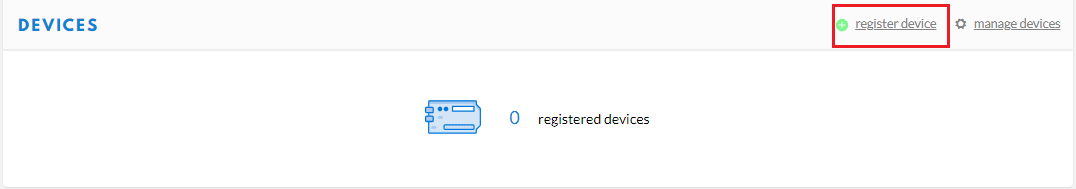
\includegraphics[width=16cm]{Bilder/lora-4.png}\\
    \caption{Übersicht der registrierten Geräte}
    \label{fig:lora-4}
\end{figure}
\begin{figure}[H]
    \center
    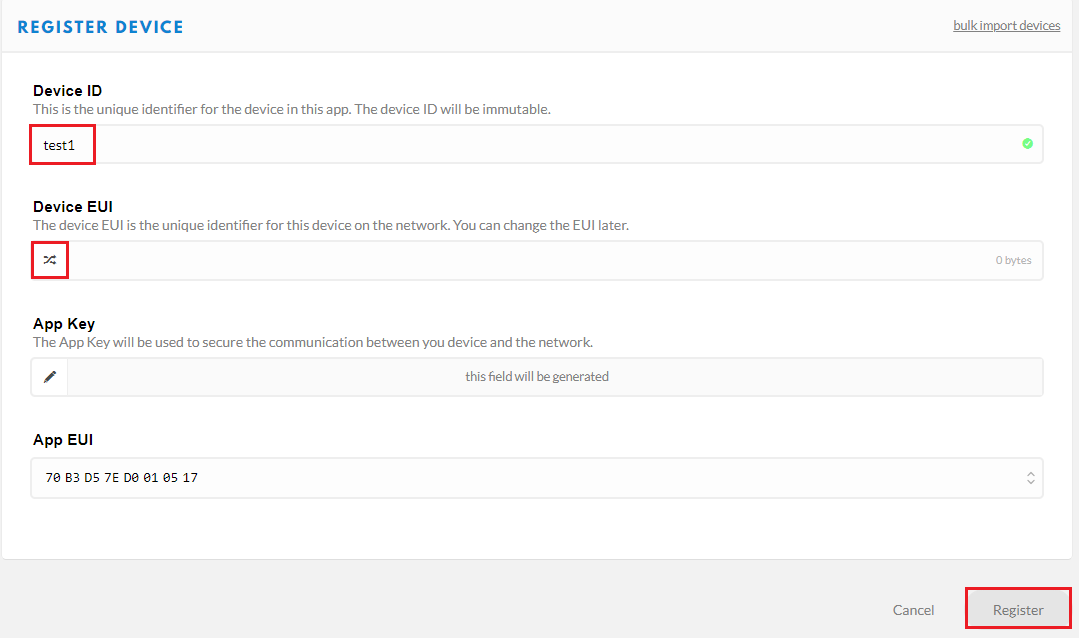
\includegraphics[width=16cm]{Bilder/lora-5.png}\\
    \caption{Formular zur Registrierung eines Geräts}
    \begin{center} \quelle\url{https://console.thethingsnetwork.org/applications} \end{center}
    \label{fig:lora-5}
\end{figure}
\newpage
\paragraph{Device ID:} Muss einzigartig sein und am besten aussagekräftig, damit man diese ID später einem Gerät zuordnen kann.

\paragraph{Device EUI:} Kann man selber bestimmen oder generieren lassen, indem man das Zufällig-Icon bzw. den Stift-Icon anklickt, um es umzuschalten. Dies wird später benötigt, um das Gerät richtig zu konfigurieren!

\paragraph{App Key:} Kann man selber bestimmen oder generieren lassen, indem man das Zufällig-Icon bzw. den Stift-Icon anklickt um es umzuschalten. Dies wird später benötigt um das Gerät richtig zu konfigurieren!

\paragraph{App EUI:} Wird automatisch generiert.\\
\\
Nachdem wir ein Gerät erstellt haben, sollten wir die Aktivierungsmethode ändern:\\
Dazu gehen wir in $Application \rightarrow application\_id \rightarrow devices \rightarrow device\_id \rightarrow Settings$. Darin kann man die Activation Method von OTAA zu ABP ändern (siehe folgende Abbildung \ref{fig:lora-6}).
\begin{figure}[H]
    \center
    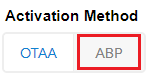
\includegraphics[width=4cm]{Bilder/lora-6.png}\\
    \caption{Aktivierungsmethoden: links Over-the-Air Activation (OTAA), rechts Activation By Personalization (ABP)}
    \begin{center} \quelle\url{https://console.thethingsnetwork.org/applications} \end{center}
    \label{fig:lora-6}
\end{figure}
\noindent
Wenn wir die Änderungen speichern, kommen wir wieder auf die Seite des Geräts. Scrollen wir ganz nach unten, dann sehen wir ein Codebeispiel (siehe folgende Abbildung \ref{fig:beispielcode}).
\begin{figure}[H]
    \center
    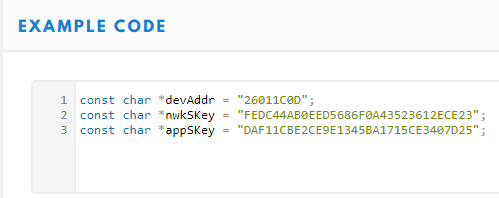
\includegraphics[width=11cm]{Bilder/lora-7.png}\\
    \caption{Beispielcode}
    \begin{center} \quelle\url{https://console.thethingsnetwork.org/applications} \end{center}
    \label{fig:beispielcode}
\end{figure}
\noindent
Diesen Codeausschnitt speichern wir oder wir merken uns, dass er auf der Seite des Geräts ist, da wir ihn später zum Konfigurieren des Nodes wieder brauchen werden. 
\section{Aufsetzen eines Clients (LoRa-Node)} \label{mac-commands}
Da unser Gateway jetzt funktionsfähig ist und wir durch die Applikation lesbare Daten erhalten können, konfigurieren wir nun die Sender (LoRa-Nodes).
Bevor wir die LoRa-Nodes mit Strom versorgen, befestigen wir erstmal eine Antenne an den RFH (Radio Frequency High Band – PIN 23) Anschluss der unsere Antenne mit 868 MHz betreiben wird.\\
Unser LoRa-Node ist über die serielle Schnittstelle UART (PIN 6 + 7 am RN2483) an den Mikrocontroller ATmega644PA (PD0 bzw. PIN 14 + PD1 bzw. PIN 15) angeschlossen und kommuniziert so mit dem Mikrochip. Die Baudrate für die UART Verbindung beträgt standardmäßig 57600 bps, kann aber auch mit einer gewissen Character Folge geändert werden (siehe folgende Abbildung \ref{fig:UART}).
\begin{figure}[H]
    \center
    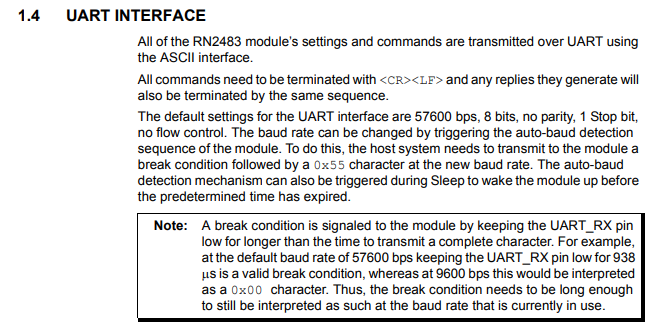
\includegraphics[width=11cm]{Bilder/lora-8.png}\\
    \caption{Spezifikationen für das UART-Interface des RN2483}
    \begin{center} \quelle\url{http://ww1.microchip.com/downloads/en/DeviceDoc/40001784F.pdf} \end{center}
        \label{fig:UART}
\end{figure}
\noindent
Kommen wir nun zur Initialisierung des RN2483, wenn dieser nun am Microchip hängt und soweit ansprechbar ist:\\

\noindent
Folgende Methoden haben wir von der Drotek RN2483 Library (\url{https://github.com/drotek/RN2483}) für Arduino genommen und für den AVR angepasst und umgeschrieben. Außerdem haben wir einen Teil von der UART-Library von unserem Betreuer Ulrich Straus übernommen.\\

\noindent
Zu aller erst setzen wir den RN2483 zurück, indem wir per UART die Befehle „\textbf{sys factoryRESET}“ und „\textbf{sys reset}“ senden und jeweils mit einem Break- und New-Line-Character bestätigen. (ASCII: Break = 0x0D; New-Line = 0x0A).\\

\noindent
Als nächstes konfigurieren wir den RN2483 mit den Daten, die wir beim Erstellen des Geräts im Applikations-Server erhalten haben. Dazu werden folgende Befehle benötigt:
\begin{itemize}
    \item \textbf{mac set devaddr <address>}
    \item \textbf{mac set nwkskey <nwksesskey>}
    \item \textbf{mac set appskey <appSesskey>}
\end{itemize}
Also mit dem Beispielcode von Abbildung \ref{fig:beispielcode} wäre dann:\\
\textbf{<address> = 26011C0D;}\\
\textbf{<nwksesskey> = FEDC44AB0EED5686F0A43523612ECE23;}\\
\textbf{<appSesskey> = DAF11CBE2CE9E1345BA1715CE3407D25}\\

\noindent
Nun müssen wir noch den \textit{Spreading Factor (siehe Kapitel \ref{sec:spreadingfactor})} festlegen und anschließend die Konfiguration speichern und dem Netzwerk beitreten.\\
Dies wird wie folgt gemacht: 

\begin{itemize}
    \item \textbf{mac set dr 5: wobei 5 = SF7/125 kHz}
    \item \textbf{mac save}
    \item \textbf{mac join abp}
\end{itemize}

\noindent
Nach jedem Befehl benutzen wir derzeit noch eine Delay-Funktion um dem RN2483 Chip Zeit zum Bearbeiten und Antworten zu lassen. Die aufgerundeten Delay-Zeiten bzw. Berechnungszeiten sieht man im folgenden Diagramm (Abbildung \ref{fig:boot-time}).

\begin{figure}[H]
    \center
    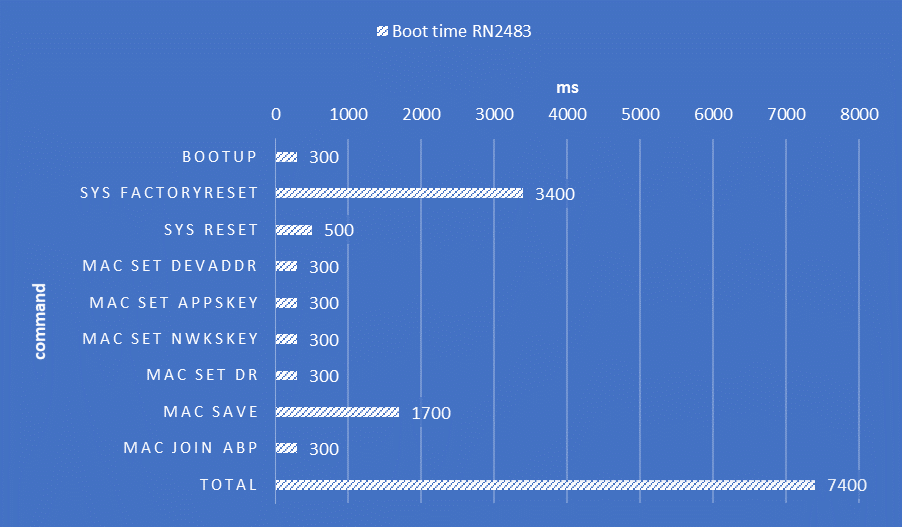
\includegraphics[width=11cm]{Bilder/lora-9.png}\\
    \caption{RN2483 Boot Time unterteilt in die einzelnen Funktionen und der benötigten Zeit in ms}
    \label{fig:boot-time}
\end{figure}
\noindent
Jetzt ist der RN2483 fertig konfiguriert und wir können mit dem Befehl „\textbf{mac tx <type> <portno> <data>}“ Nachrichten versenden. Dabei ist:\\

\textbf{<type>} = cnf (confirmed) oder uncnf (unconfirmed);\\

\textbf{<portno>} = Portnummer zwischen einschließlich 1 und 223;\\

\textbf{<data>} = Die Nachricht als Hexadezimal Wert.\\
\noindent
Die vollständige Kommandoliste mit Syntax und Rückgabewerten findet man im RN2483 LoRa Technology Module Command Reference User’s Guide: \url{http://ww1.microchip.com/downloads/en/DeviceDoc/40001784F.pdf}\\
Wir benötigen aus dieser Liste nur die System Commands aus Kapitel 2.3 und die MAC Commands aus Kapitel 2.4

\section{Spreading Factor} \label{sec:spreadingfactor}
Der LoRa-Knoten (LoRa-Node) ist nun bereit die Gewichtsinformationen über die Kaffeekanne entgegenzunehmen und als Nachricht verpackt zu senden.
Nun geht es um die Feinabstimmung der Konfiguration, um die Reichweite und die Bandbreite des LoRa-Knotens zu bestimmen.\\
Spreading Factor (kurz: SF) ist, wie der Begriff teilweise schon verrät, ein Faktor, der angibt wie weit sich eine versendete Nachricht ausbreitet, also was für eine Reichweite sie hat. Umso höher dieser Faktor, desto höher die Reichweite. Jedoch leidet die Geschwindigkeit der Übertragung darunter. Man kann sich merken: 
\begin{itemize}
    \item kleiner SF = hohe Bitrate, nicht so hohe Reichweite;
    \item hoher SF = niedrige Bitrate, hohe Reichweite.
\end{itemize} 
In der folgenden Tabelle (Abbildung \ref{fig:spreading-factor}) ist dies sehr gut erkennbar. 
\begin{figure}[H]
    \center
    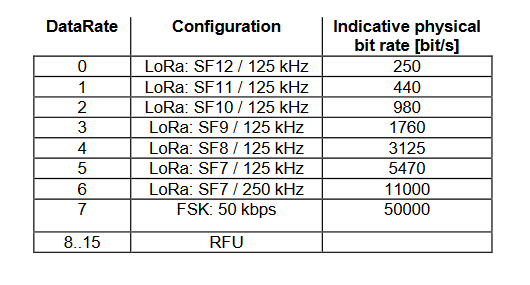
\includegraphics[width=15cm]{Bilder/lora-10.png}\\
    \caption{Tabelle mit verschiedenen Spreading Factors und die zugehörige Bitrate}
    \begin{center} \quelle\url{https://witekio.com/wp-content/uploads/2018/01/lora-wan-spreading-factor.png} \end{center}
        \label{fig:spreading-factor}
\end{figure}
\noindent
Derzeit sind unsere Payloads (Nachrichten) durchschnittlich nur 2 Bytes lang, da wir nur den Füllstand übermitteln. Beim SF7 könnten wir 647 Nachrichten am Tag senden, wenn wir unter dem 30 Sekunden Sendelimit bleiben wollen.\\

\noindent
Die genaue Berechnung und weitere Infos zum Spreading Factor findet man auf folgender Google Docs Tabelle: \url{https://docs.google.com/spreadsheets/d/1QvcKsGeTTPpr9icj4XkKXq4r2zTc2j0gsHLrnplzM3I/edit}

\section{Security / Datensicherheit}
Jedes gute System sollte vor Angreifern geschützt sein. Und das ist auch bei LoRaWAN von TheThingsNetwork der Fall. Die Nachrichten werden vor dem Versenden verschlüsselt und beim Empfänger mit Hilfe des App-Session-Key entschlüsselt. Nachrichten von LoRa-Knoten werden als lesbare digitale Daten über ein Frequenzband übermittelt. Da die Frequenzen bekannt sind, kann jeder die Nachrichten abfangen und mitlesen. Die Mitleser sind aber durch die Verschlüsselung nicht in der Lage den Inhalt zu verstehen. Über einen Replay-Angriff (siehe Wikipedia \url{https://de.wikipedia.org/wiki/Replay-Angriff}) könnte der Interessent sich beim Empfänger aber als jemand anderen ausgeben und so die Entschlüsselung erfahren. Als Maßnahme, um gegen diese Art von Angriff zu schützen, wird ein Frame Counter eingesetzt der jedes Mal, wenn eine Nachricht versendet wird sich um 1 erhöht. So werden alle alten Nachrichten ignoriert und man ist vor Replay-Angriffen geschützt.\\

\noindent
Weitere Infos hierzu gibt es auf der TheThingsNetwork Seite zu Security: \url{https://www.thethingsnetwork.org/docs/lorawan/security.html}

\section{Methoden und Funktionen zur Kommunikation mit dem LoRa-Modul (UART \& Modul RN2483)}
Nachdem die LoRa-Kommunikation nun sicher ist, wurde der reibungslose Ablauf im LoRa-Knoten, also zwischen dem LoRa-Modul (RN2483) und dem Mikrocontroller (ATmega644PA), sichergestellt.
Die serielle Schnittstelle (UART), die zwischen beiden Bauteilen besteht, implementiert die Methoden des RN2483 für die getaktete Übertragung zum Gateway.
\subsection{RN2483.c}
\begin{itemize}
    \item \textbf{RN2483\_init():} Initialisiert / Konfiguriert das RN2483 Modul wie im Codebeispiel \ref{lst:payload} zu sehen ist.
    \item \textbf{RN2483\_sendData(char *s):} Konvertiert mit sendHex2(s) das gewünschte Char-Array in Hexadezimal ASCII Code und sendet es mit der UART-Schnittstelle an das Modul, welches anschließend die Nachricht über LoRaWAN an das Gateway schickt.
    \item \textbf{RN2483\_sendCmd(char *cmd):} Sendet ein Kommando über die UART-Schnittstelle an das Modul.
    \item \textbf{RN2483\_prepareMessage(int fillRatio):} Konvertiert ein Integer Wert in Hexadezimal ASCII Code und sendet es über die UART-Schnittstelle an das Modul, welches anschließend die Nachricht über LoRaWAN an das Gateway schickt.
    \item \textbf{delayFunction(int number):} Führt einen Delay aus, da bei uns maximal nur 850ms am Stück mit der Delay Funktion gewartet werden kann. Bei Parameter-Wert 1 wird 3400ms gewartet, bei 2 wird 500ms gewartet, bei 3 wird 300ms gewartet und bei 4 wird 1700ms gewartet. 
\end{itemize}
\subsection{uart.c}
\begin{itemize}
    \item \textbf{init\_uart():} Initialisiert die UART-Schnittstelle im Mikrocontroller, d.h. setzt die Baudrate, aktiviert die RX und TX Pins und setzt den asynchronen UART Modus mit 8 Data bits, no parity, 1 stop bit. 
    \item \textbf{uart\_putc(unsigned char c):} Sendet einen Buchstaben über UART, wenn die Schnittstelle bereit ist.
    \item \textbf{sendString(char tempStringChar[]):} Sendet ein Char-Array über UART, indem es für jeden Char die uart\_putc() Methode aufruft. 
    \item \textbf{sendHex2(char *s):} Konvertiert das gegebene Char-Array in Hexadezimal ASCII Code und sendet es über die sendString() Methode.
\end{itemize}
\newpage


\chapter{Webserver für die Visualisierung}
\section{Visualisierung der empfangenen Daten mit Angular CLI}
Mit dem aufgesetzten Gateway, welches die Gewichtsdaten/Füllstände über verschlüsselte Kanäle ins Internet überträgt, fehlt noch die Komponente der Visualisierung. Der Webserver, der den Clients die Weboberfläche (das Front-End) zur Verfügung stellt, übernimmt die Aufgabe der Aufbereitung und Darstellung der übermittelten Daten.
Das Front-End ist die Ansicht, auf welche der Kunde blickt, um die Füllstände aller Behälter zu sehen. Sie ist minimalistisch gehalten, sodass keine Überladung entsteht und das menschliche Auge die relevante Information schneller erkennt. \\
\begin{figure}[H]
    \center
    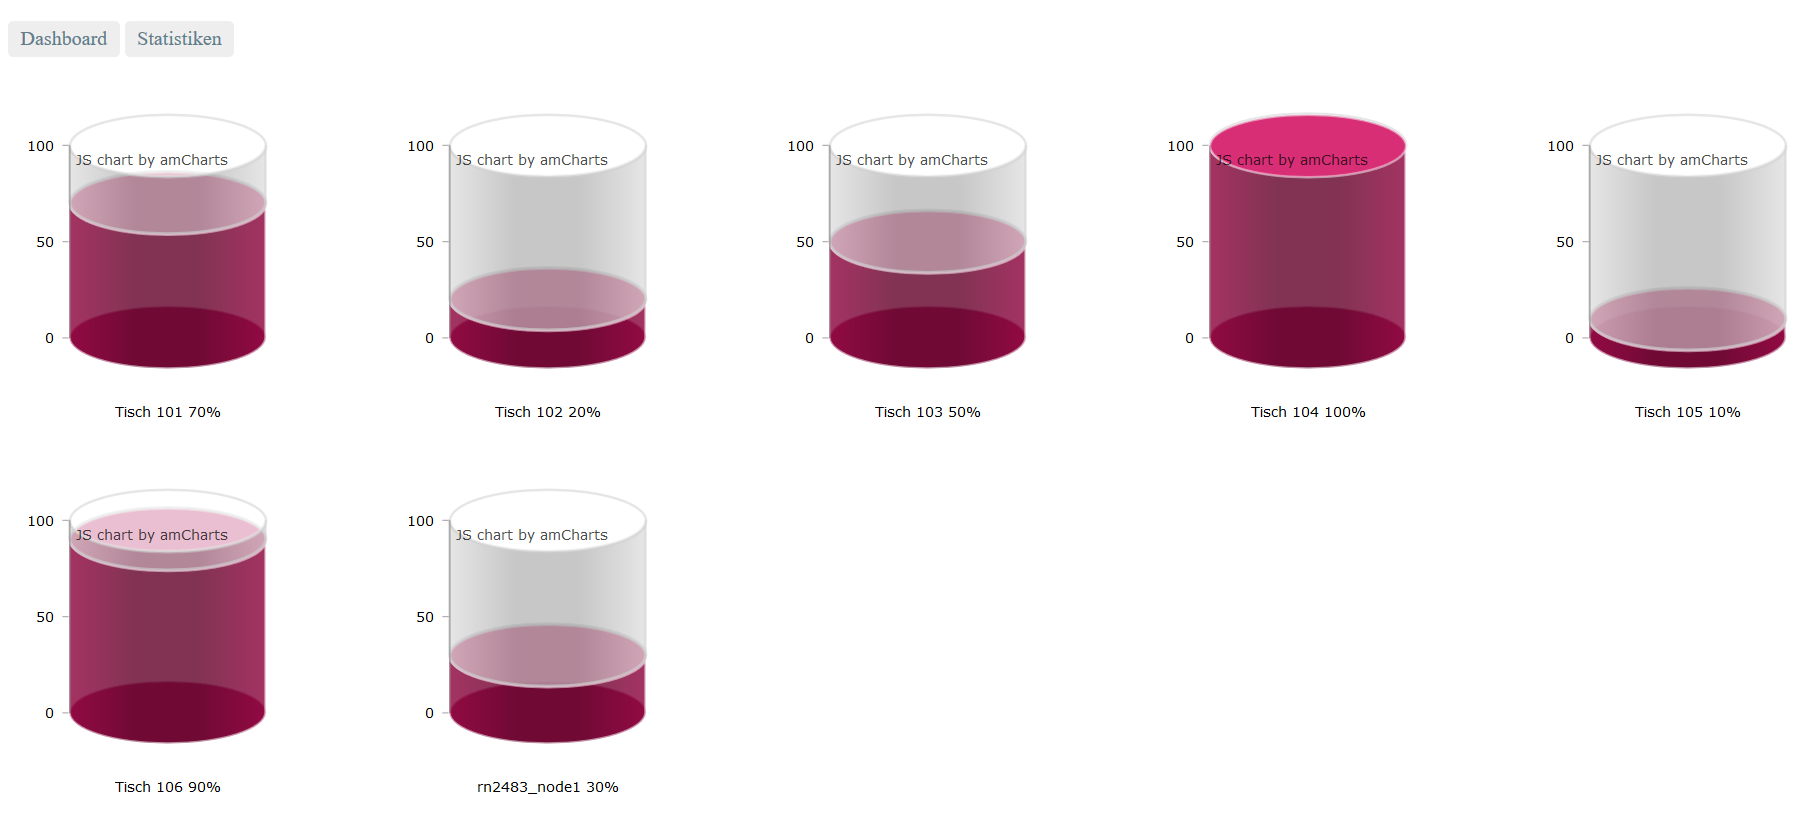
\includegraphics[width=16cm]{Bilder/front-end-1.png}\\
    \caption{Übersicht der Füllstände der einzelnen Kaffeemaschinen auf der Webseite}
    \label{fig:front-end-1}
\end{figure}
\noindent
Die Webseite (siehe Abbildung \ref{fig:front-end-1}) zeigt links oben zwei Buttons, die zwischen zwei Anzeigen hin- und herschalten lassen. Die eigentliche Haupt- bzw. Startseite (Dashboard - siehe Abbildung \ref{fig:front-end-1}) mit den Zylindern und deren Inhalten
- jeder aktive Node wird hier mit seinem aktuellen Füllstand angezeigt. Und die Statistik-Seite (siehe Abbildung \ref{fig:front-end-2}), die auf einem größeren Diagramm die historischen Werte
bis zum aktuellen Zeitpunkt anzeigt.
\begin{figure}[H]
    \center
    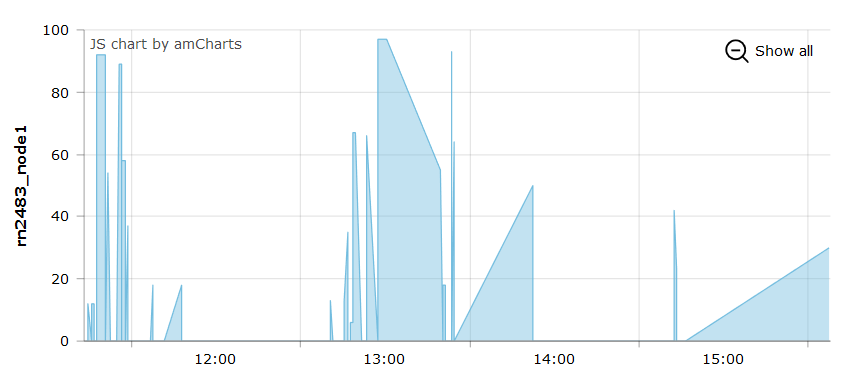
\includegraphics[width=16cm]{Bilder/front-end-2.png}\\
    \caption{Füllstand-Verlauf einer Kaffeemaschine von 12:00 Uhr bis 15:00 Uhr}
    \label{fig:front-end-2}
\end{figure}
\noindent
Die Visualisierung ist mithilfe des Front-End-Frameworks Angular CLI geschrieben worden. Die Programmiersprache von Angular ist TypeScript, eine Weiterentwicklung von JavaScript, mit einigen Verbesserungen wie die Typisierung von Variablen. Weiterhin wurden die Zylinder-Behälter mit der „AmCharts“ Angular-Bibliothek implementiert. Diese Bibliothek bietet die Möglichkeit diese Diagramme mit Hilfe einer „create“ Funktion zu erstellen und einer „update“ Funktion mit neuen Daten zu versorgen und damit das Diagramm in Echtzeit zu verändern. Darüber hinaus wurden die Statistikdiagramme mit Hilfe der gleichen Bibliothek erstellt. Diese Diagramme bieten die gleichen Funktionen wie die Zylinderdiagramme.

\newpage
\section{The Things Network}
Das Things Network ist ein globales, freies und dezentrales Internet der Dinge Netzwerk. Es hat sich zum Ziel gesetzt, ein weltweit offenes und unabhängiges Internet der Dinge Netzwerk aufzubauen.

\begin{figure}[H]
    \center
    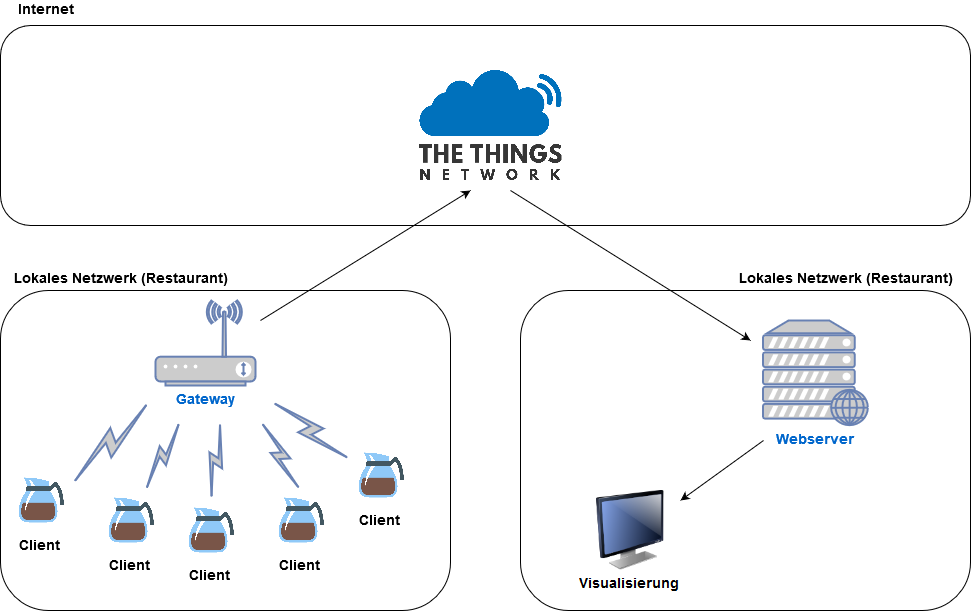
\includegraphics[width=16cm]{Bilder/Netzwerkdiagramm.png}\\
    \caption{Netzwerkdiagramm}
    \label{fig:Netzwerkdiagramm}
\end{figure}

\section{Verarbeitung der Datenpakete}
Um die Daten, die an das ``TheThingsNetwork'' geschickt werden, in unserem Webserver überhaupt zu empfangen, ist die Verbindung zwischen den beiden unerlässlich. Dazu wurde ein Server aufgesetzt, der in der Programmiersprache Node.js geschrieben ist und in direktem Kontakt mit TheThingsNetwork steht. Dieser Webserver setzt das Server-Framework ``Express.js'' ein und nutzt einen Websocket, um die übertragenen Messdaten von TheThingsNetwork zu erhalten. Während der Verarbeitung der Daten, übernimmt der Webserver außerdem den Prozess der Persistierung.\\

\noindent
Damit eine Verbindung zwischen den beiden Servern hergestellt werden kann, müssen im Voraus zwei Werte vorhanden sein. Der erste Wert ist die Application ID. Diese ID beschreibt das Projekt, welches vorher bei der TheThingsNetwork Webseite festgelegt wurde. In diesem Fall ist die Application ID: \textit{lora\_measure\_network}. Der zweite Wert ist der \textit{accessKey}. Dieser Wert ist für die Authentifizierung mit dem Netzwerkserver erforderlich. Der \textit{accessKey} muss vorher über die Webseite generiert werden. Dabei folgen die Nachrichten zwischen den Servern einem bestimmten Format:\\


\begin{lstlisting}[caption=Einkommender Messdatensatz,label=lst:payload]
    { 
        app_id: 'lora_measure_network',
        dev_id: 'rn2483_node1',
        hardware_serial: '0004A30B001C6A30',
        port: 1,
        counter: 0,
        payload_raw: <Buffer 33 30>,
        metadata: { time: '2018-07-05T18:04:13.482082016Z' },
        message: '30' 
    }
\end{lstlisting}
\begin{itemize}
    \item \textbf{app\_id:} Application ID
    \item \textbf{dev\_id:} Das Gerät, welches die Nachricht gesendet hat 
    \item \textbf{hardware\_serial:} Hardwarenummer des Nodes
    \item \textbf{counter:} Messagecounter der bei jeder Nachricht um 1 inkrementiert
    \item \textbf{payload\_raw:} Die Nachricht wird vom Network Server als Hexadezimal
    \item \textbf{metadata:} In diesem Objekt ist ein Zeitstempel enthalten. Dieser Zeitstempel ist von dem Zeitpunkt, als die Nachricht im Network Server angekommen ist.
    \item \textbf{message:} Das ist die Payload, welche vom payload\_raw geparst wurde 
\end{itemize} 
\newpage
\section{Inaktivität der Behälter}
Sobald ein Gerät inaktiv wird (d.h. eine Stunde ohne Nachrichtenempfang), ist es für die Nutzer in der UI nicht mehr möglich, das Gerät zu sehen. Diese Inaktivität würde bei einem Thermobehälter die Abkühlung bedeuten. Diese Zeitbeschränkung wurde nach einer Gesprächsrunde innerhalb der Entwickler festgesetzt.\\
Falls das Gerät unerwartet vom Netz genommen wird, kann das in der Visualisierung für Verwirrung sorgen. Tritt dieser Fall ein, könnte man auf der Webseite, auf der die Behältnisse angezeigt werden, nicht erkennen, ob das Gerät überhaupt noch existiert. Deshalb wird das Gerät, sobald es wieder im Netz ist, mit den aktuellen Messwerten in der UI eingeblendet. 

\section{Voraussetzungen und Nutzung des Webservers}
Um den Webserver, der für die Kommunikation hin zu den Knoten-Daten und die Visualisierung für die Gastro-Mitarbeiter, im realen Umfeld betreiben zu können, sind für das Aufsetzen folgende Systeme/Software notwendig.\\

\noindent
\textbf{Unterstützte Betriebssystem}
%Überleitung wie in Kommentar von ulli
\begin{itemize}
    \item Windows
    \item Linux
    \item Unix
\end{itemize} 
\textbf{Benötigte Software}
\begin{itemize}
    \item Node.js
    \item Angular
\end{itemize} 
\textbf{Nutzung}
\begin{itemize}
    \item Starte zwei Kommandozeilenprogramme und führe die Befehle aus:
    \begin{itemize}
        \item Konsole 1 im Ordner „server“: \textit{node server.js} 
        \item Konsole 2 im Ordner „client“: \textit{ng serve --open}
    \end{itemize}
\end{itemize} 
\newpage
\chapter{Schaltplan und Verlöten der Platine}
Nachdem alle Komponenten nun miteinander interagieren, wurde zum Abschluss der LoRa-Knoten, der bisher aus Entwicklungsboards und Modulen zusammengesteckt war, in eine eigene Platine verwandelt. Ein designter Schaltplan half die Einzelteile auf einer Lochrasterplatine zu verlöten.\\
Der Schaltplan wurde mit dem Programm Fritzing (\url{http://fritzing.org/home}) erstellt.
\begin{figure}[H]
    \center
    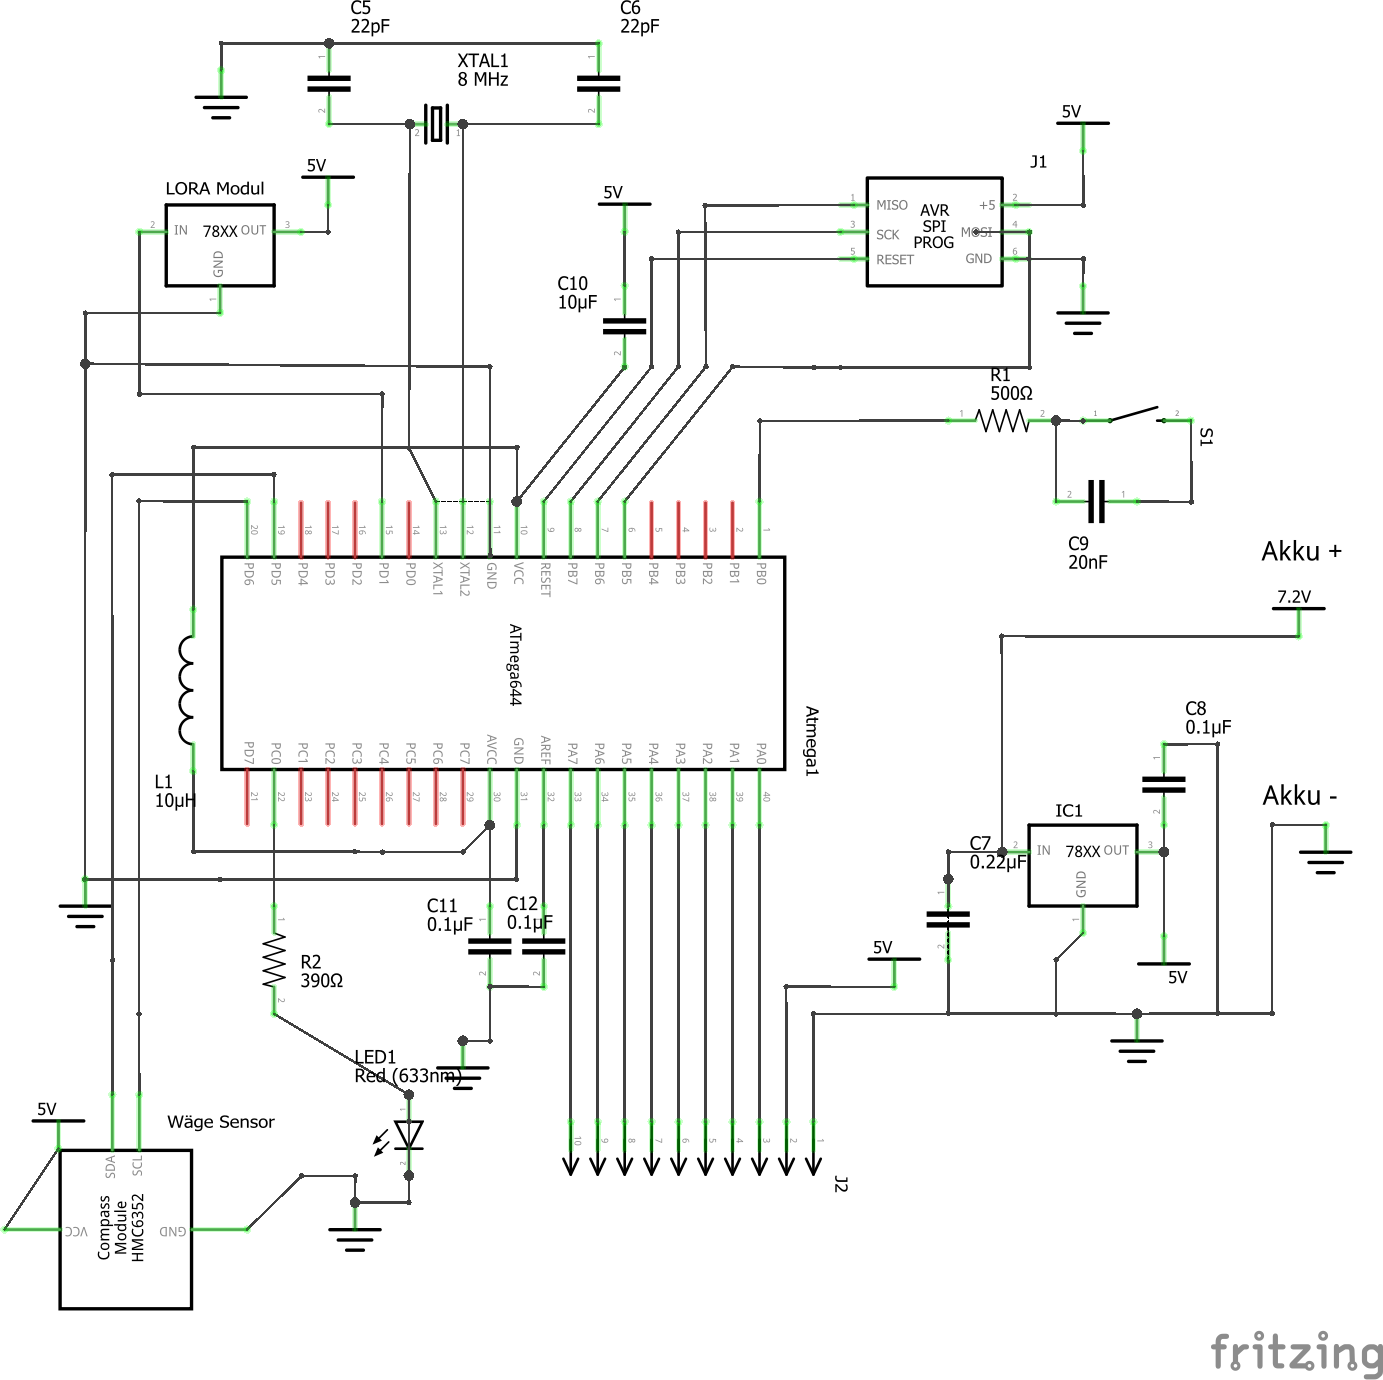
\includegraphics[width=15cm]{Bilder/schaltplan-1.png}\\
    \caption{Schaltplan, erstellt mit Fritzing}
    \label{fig:schaltplan}
\end{figure}
\newpage
\noindent
Als Mikrocontroller haben wir im Schaltplan einen ATmega644 statt einem ATmega644PA verwendet, da diese fast gleich sind. Ausgehend vom Mikrocontroller werden an den Pins XTAL1 und XTAL2 der Quarz angeschlossen. Die Pins PA0 bis PA7 sind für ein LCD Display reserviert, auf dem Gewichtsinformationen, aber auch Debug-Meldungen ausgegeben werden können. Der Wägesensor ist mit den Pins PD5 und PD6 verbunden. Wobei hier noch die notwendigen Pullup-Widerstände für die I\textsuperscript{2}C- (Two-Wire-) Schnittstelle fehlen. Für das Wägesensor-Bauteil (im Schaltplan fälschlicherweise als Compass, HMC betitelt) wurde ein Platzhalter-Bauteil mit vier Pins verwendet, da kein passendes Layout für unseren Wägesensor gefunden wurde. Das LoRa-Modul wird an PD1 angeschlossen und es wurde ebenso eine Platzhalterkomponente mit drei Pins verwendet. Zudem haben wir einen Taster auf PD0 für die direkte Kommunikation mit dem Wäge-Modul und an PD5 – PD7 einen ISP-Anschluss für die Programmierung angelötet. Die Platine und dessen Bauteile werden mit zwei in Reihe geschalteten Akkus versorgt die jeweils eine Spannung von ca. 3,6 Volt haben und damit eine Gesamtspannung von 7,2 Volt liefern. Dazwischen geschaltet ist ein DC-DC Wandler, der den Stromkreis auf konstante 5V versorgt.\\

\noindent
Die Rückseite der gelöteten Platine:
\begin{figure}[H]
    \center
    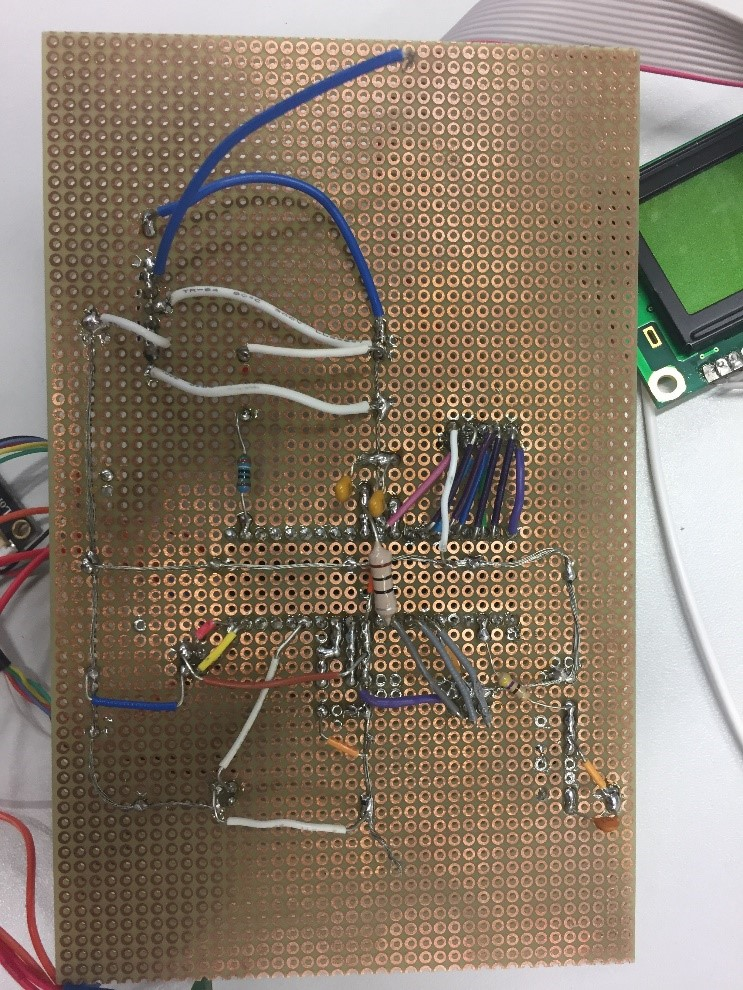
\includegraphics[width=10cm]{Bilder/schaltplan-2.jpg}\\
    \caption{Rückseite der verlöteten Platine unseres ersten Prototyps}
    \label{fig:schaltplan-rueckseite}
\end{figure}
\begin{figure}[H]
    \center
    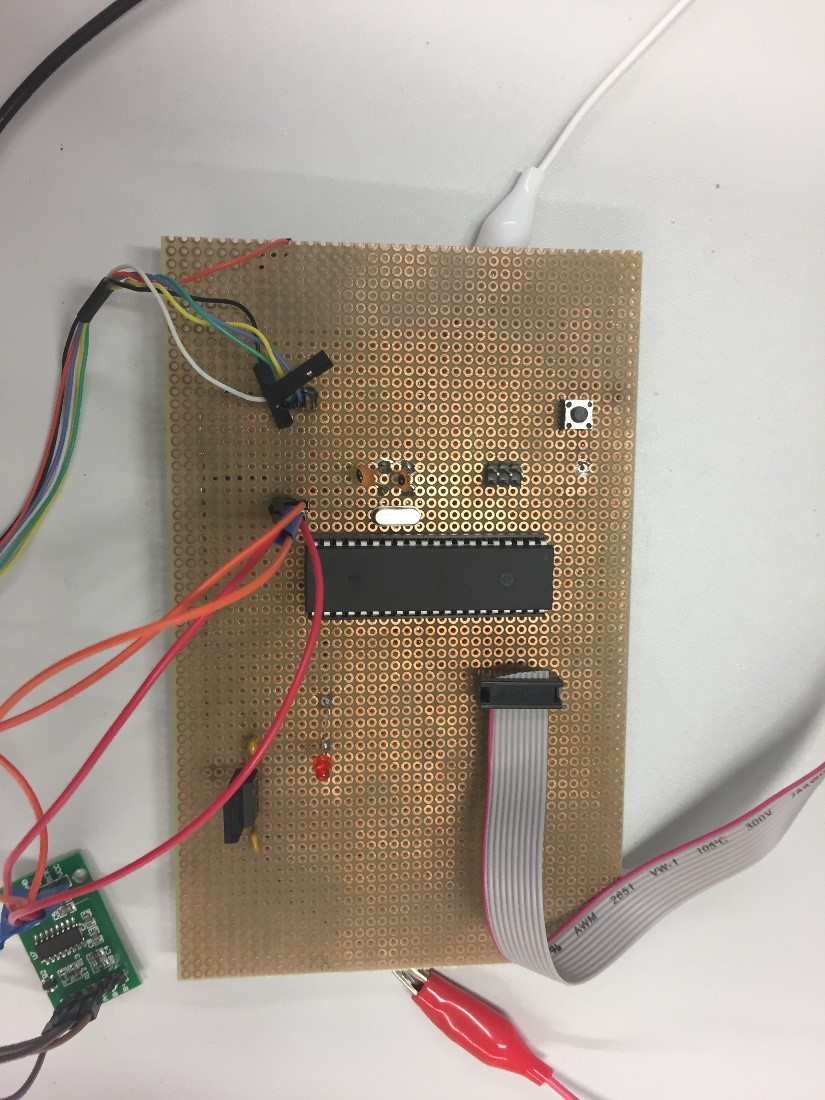
\includegraphics[width=10cm]{Bilder/schaltplan-3.jpg}\\
    \caption{Vorderseite der verlöteten Platine unseres ersten Prototyps}
    \label{fig:schaltplan-vorderseite}
\end{figure}
\noindent
Dem Taster wurde eine Tar-Funktion zugewiesen, mit der das Gewicht genullt werden kann. Softwareseitig ist es auch möglich dem Taster andere Funktionen zuzuweisen, wie beispielsweise das An- und Ausschalten des Gerätes oder mit Verbund eines Displays zwischen verschiedenen Anzeigemodi zu wechseln.

\chapter{Fazit der prototypischen Umsetzung eines Wägesystems für den Gastronomie-Betrieb via LoRaWAN}
Zusammenfassend sei zu sagen, dass der Aufbau, die Funktion und der Nutzen der angenommenen Vorteile vollumfänglich realisiert werden konnte.\\
Alle Komponenten arbeiten nach Konfiguration und Implementierung exakt so zusammen, dass der reibungslose Ablauf des Prozesses der ständigen Visualisierung von Füllstand und dem Nachfüllen der Behältnisse gewährleistet ist.\\
LoRa bietet über verschiedene Kommunikationswege eine sichere, energieeffiziente Übertragung und kann alle nötigen Daten zur Visualisierung übermitteln. Die Zyklen, die zur Übermittlung zu Verfügung stehen, sind ausreichend kurz damit die nutzbaren Informationen, also Füllstände von Kaffeebehältnissen oder anderen Behältnissen, clientseitig in Echtzeit zu sehen sind. Wobei der Energieverbrauch im Einzelnen nicht untersucht wurde, konnten Beobachtungen an den verwendeten Akkupacks Rückschlüsse auf die enorm niedrigen Energiekosten zulassen.\\
Für eine weiträumige Nutzung, konnten Tests anderer Gruppen zeigen, dass selbst in riesigen Gastro-Anlagen die nötigen Reichweiten erzielt werden können, die für eine Füllstands-Anwendung nötig sind.\\
Zudem läuft das System plattformunabhängig, sodass man das System auf vielen verschiedenen Geräten verwenden kann. Die Visualisierung wird im Browser, beispielsweise Internet Explorer oder Google Chrome angezeigt, sodass keine weiteren Installationen nötig sind. Der Server läuft auch auf diversen Betriebssystemen wie Windows oder MacOS, sodass hier keine großen Umstellungen nötig sind. Außerdem ist es auch möglich die Visualisierung auf einem Smartphone aufzurufen, beispielsweiße auf einem iPhone, da diese auch einen Browser installiert haben, sodass man die Füllstande auch zwischendurch und schnell überprüfen kann.\\
Dadurch, dass das System plattformunabhängig implementierbar ist, kann man es unkompliziert und flexibel in ein bestehendes System des Hotels oder Gastronomie integrieren. Eine mögliche Option ist, dass man den Raspberry Pi an einen PC anschließt und eine Installation startet, damit die ganzen Systeme installiert und hochgefahren werden. \\
Abschließend muss erwähnt werden, dass ein großes Verbesserungspotential vorhanden ist, sodass weitere nützliche Funktionen eingebaut werden können, damit die Prozesse in der Gastronomie und in Hotels verbessert werden.

\chapter{Ausblick auf die Kommerzialisierung}
\section{LoRaWAN Modul Code verbessern}
\begin{itemize}
    \item Firmware vom \textbf{RN2483} updaten
    \item Gebrauch von der sleep Funktion „sys sleep <length>“ machen um Strom zu sparen
    \item Beim Ausschalten den Frame-Counter mit „mac get upctr“ auslesen und in den EEPROM vom ATmega644PA speichern. Beim Einschalten den Frame Counter aus dem EEPROM auslesen und mit „mac set upctr <fCntUp>“ wieder neu setzen, damit man nicht jedes Mal den Frame Counter in der Konsole von TheThingsNetwork zurücksetzen muss. 
    \item Empfang von Nachrichten oder Befehlen vom Gateway ermöglichen und durch UART-Receive diese Nachrichten bzw. Befehle im Mikrocontroller auslesen. 
    \item Delays durch Interrupts ersetzen, so dass das Programm weiterarbeiten kann, während es auf ein Ereignis wartet.
    \item Verschiedene Profile oder Modis passend zu den \textit{Spreading Factors (siehe Kapitel \ref{sec:spreadingfactor})} programmieren z.B.: niedrige Reichweite + hohe Bandbreite, hohe Reichweite + niedrige Bandbreite, etc.
\end{itemize} 
\section{Front-End Lizenzkosten vermeiden}
Das Front-End hat das Problem, dass es die „AmCharts“-Bibliothek nutzt. Die Bibliothek ist für Open-Source- und nicht-kommerzielle Projekte frei verfügbar. Die Lizenz (Stand 06.07.2018) kostet für ein Jahr 4590 \euro. Darin sind die Diagramme in den Seiten Dashboard und Statistik enthalten. In Zukunft sollen selbstentwickelte Diagramme verwendet werden, um Lizenzkosten zu vermeiden.
\newpage
\section{Erstellen eines wasserfesten Gehäuses}
In naher Zukunft ist es außerdem noch wichtig, dass sich die Platine und die nötige Hardware in einem Gehäuse befinden, da es sonst nicht im kommerziellen Umfeld nutzbar wäre. Zudem sollte das Gehäuse wasserfest sein, da sonst Kaffee oder ähnliches hindurchkommen und etwas beschädigen könnte.\\

\noindent
Dadurch wird unser Produkt deutlich kompakter und nutzvoller für Hotels. Unser erster Ansatz wäre ein Prototyp mit einem 3D-Drucker zu erstellen. 
\section{Kommerzialisierung und mögliches Geschäftsmodell}
Die nächsten nötigen Schritte zur Kommerzialisierung sind:
\begin{enumerate}
    \item Kundengespräche:\\
    Wir müssen Gespräche mit unseren potenziellen Kunden, beispielsweise Hotels oder Restaurants führen, damit wir abschätzen können, wie hoch die Nachfrage sein könnte. Hierbei bekommen wir direktes Feedback zu unseren Prototypen, sodass darauf reagiert werden kann. Außerdem müssen wir Kundengruppen erschließen, damit wir eingrenzen können, in welchen Branchen das Produkt nutzbar ist.
    \item Optimierung des Prototyps:\\
    Wir müssen ein wasserdichtes Gehäuse erstellen, damit die Technik verpackt werden kann. Zudem muss das Design des Gehäuses angepasst werden, sodass es in der Gastronomie verwendbar ist. Des Weiteren werden wir den Prototypen verbessern, indem wir einen Sleep-Mode einführen, damit die Laufzeit verlängert wird, den Taster verbessern und unnötige Komponenten entfernen.
    \item Erstellen von Business-Plan, Strategie und Dokumente für Unternehmensgründung:\\
    Für eine erfolgreiche Start-Up-Gründung benötigen wir einen Business-Plan, damit wir einen seriösen roten Faden haben und wir damit Investoren überzeugen können. Zudem müssen wir uns Strategien überlegen und die nächsten Schritte planen. Dazu benötigen wir noch weitere Dokumente und Berechnungen für die Unternehmensgründung.
\end{enumerate}

\noindent
Mögliches Geschäftsmodell: \\
Um den Aufwand für Gastronomiebetreiber möglichst klein zu halten, sollten Geräte- und Softwarewartung möglichst outgesourct sein. 
Gastronomiebetreiber bezahlen monatlich/jährlich für die Nutzung des Systems eine festgelegte Summe. 
Darin sind Installationen und Wartungsarbeiten enthalten. Für Erweiterungen und/oder Updates fallen weitere Einmalgebühren und eventuell Aufschläge im jährlichen Turnus an. Der Server wird im cloudbasierten Betrieb realisiert, was Wartung und Updates der lokalen Installationen vereinfacht. Lediglich der Austausch und die initiale Installation vor Ort macht einen Besuch nötig.

\nocite{online:getting-started-load-cells}
\nocite{doc:getting-started}
\nocite{wiki:load-cell}
\nocite{wiki:Force-sensing-resistor}
\nocite{wiki:Piezoelectric-sensor}
\nocite{online:ic880a-gateway}
\nocite{online:datalink}
\nocite{online:lorawan-security}
\nocite{excel:lorawan-airtime}
\nocite{picture:spreading-factor}
\nocite{picture:lorawan}
\nocite{doc:rn2483}
\nocite{doc:lora-documentation}

\printbibliography
\end{document}